%%%%%%%%%%%%%%%%%%%%%%%%%%%%%%%%%%%%%%%%%%%%%%%%%%%%%%%%%%%%%%%%%%%%%%%%%%%%%%%%%%%
%%                                                                               %%
%% Document author: Moises Chavez-Martinez                                       %%
%%                                                                               %%
%% Description: This document is intended to be a technical and user manual for  %%
%%              the reader. In this document will be explained all the possible  %%
%%              details about the LibOpenCIF library.                            %%
%%                                                                               %%
%% --- Resources ---                                                             %%
%%                                                                               %%
%% This document is based on The Legrand Orange Book LaTex template:             %%
%% http://www.latextemplates.com/template/the-legrand-orange-book                %%
%%                                                                               %%
%% The icons used in the notes for the document (the Info, Warning               %%
%% and Error icons) where originally found at these sites:                       %%
%% http://www.iconsdb.com/green-icons/info-icon.html                             %%
%% http://www.iconsdb.com/orange-icons/warning-5-icon.html                       %%
%% http://www.iconsdb.com/red-icons/error-5-icon.html                            %%
%%                                                                               %%
%% Front cover image found at these sites:                                       %%
%% http://www.muycomputer.com/files/HIDDEN_264_19888_FOTO_Intel_4004_esquema.jpg %%
%% http://www.trecut.wellcome.ro/?p=3537                                         %%
%%                                                                               %%
%%%%%%%%%%%%%%%%%%%%%%%%%%%%%%%%%%%%%%%%%%%%%%%%%%%%%%%%%%%%%%%%%%%%%%%%%%%%%%%%%%%

%%%%%%%%%%%%%%%%%%%%%%%%%%%%%%%%%
%%                             %%
%% PREAMBLE AND FIRST COMMANDS %%
%%                             %%
%%%%%%%%%%%%%%%%%%%%%%%%%%%%%%%%%

\documentclass[11pt,twoside,openany,x11names,svgnames]{memoir}

\usepackage{lmodern}
\usepackage{wallpaper}
\usepackage{tikz}
\usepackage{listings}
\usetikzlibrary{shapes,positioning}

\usepackage[utf8]{inputenc}

\usepackage[english]{babel}
\selectlanguage{english} 

%% Custom stock paper and page size
\setstocksize{279mm}{216mm}
\settrimmedsize{\stockheight}{\stockwidth}{*}

%% Adjust margins around typeblock
\setlrmarginsandblock{23mm}{18mm}{*}
\setulmarginsandblock{23mm}{23mm}{*}

%% Header and footer heights
\setheadfoot{\baselineskip}{10mm}
\setlength\headsep{7mm}

%% To apply and enforce layout
\checkandfixthelayout

%% Command to hold chapter illustration image
\newcommand\chapterillustration{}

%% Define a fancy chapter style
\makechapterstyle{FancyChap}{
	%% Vertical Space before main text starts
	\setlength\beforechapskip{0pt}
	\setlength\midchapskip{0pt}
	\setlength\afterchapskip{137mm}
	%% Will print chapter number and title
	%% in one go ourselves
	\renewcommand*\printchaptername{}
	\renewcommand*\printchapternum{}
	%%% Re-define how the chapter title is printed
	\def\printchaptertitle##1{
		%% Background image at top of page
		\ThisULCornerWallPaper{1}{\chapterillustration}
		%% Draw a semi-transparent rectangle across the top
		\tikz[overlay,remember picture]
	  	\fill[fill=LimeGreen,opacity=.7]
			(current page.north west) rectangle 
			([yshift=-3cm] current page.north east);
		%% Check if on an odd or even page
		\strictpagecheck\checkoddpage
		%% On odd pages, "logo" image at lower right
		%% corner; Chapter number printed near spine
		%% edge (near the left); chapter title printed
		%% near outer edge (near the right).
		\ifoddpage{
		    \begin{tikzpicture}[overlay,remember picture]
			    \node[anchor=south west,
					xshift=20mm,yshift=-30mm,
					font=\sffamily\bfseries\huge] 
  	 	   			at (current page.north west) 
 	  	   			{\chaptername\chapternamenum\thechapter};
 	  	 		\node[fill=ForestGreen!80!black,text=white,
 	  	   			font=\Huge\bfseries, 
 	  	   			inner ysep=12pt, inner xsep=20pt,
 	     			rounded rectangle,anchor=east, 
 	     			xshift=-20mm,yshift=-30mm] 
 	     			at (current page.north east) {##1};
 		   	\end{tikzpicture}
 	 	}
	  	%% On even pages, "logo" image at lower left
  		%% corner; Chapter number printed near outer
  		%% edge (near the right); chapter title printed
  		%% near spine edge (near the left).
  		\else{
   	 		\begin{tikzpicture}[overlay,remember picture]
    			\node[anchor=south east,
      				xshift=-20mm,yshift=-30mm,
      				font=\sffamily\bfseries\huge] 
      				at (current page.north east)
      				{\chaptername\chapternamenum\thechapter};
    			\node[fill=ForestGreen!80!black,text=white,
      				font=\Huge\bfseries,
      				inner sep=12pt, inner xsep=20pt,
      				rounded rectangle,anchor=west,
      				xshift=20mm,yshift=-30mm] 
      				at ( current page.north west) {##1};
    		\end{tikzpicture}
  		}
  		\fi
	}
}


%% Define a fancy chapter style for unnumbered
%% chapters (e.g. the Table of Contents)
\makechapterstyle{FancyUnnumberedChap}{
	%% Vertical Space before main text starts
	\setlength\beforechapskip{0pt}
	\setlength\midchapskip{0pt}
	\setlength\afterchapskip{47mm}
	%% Will print chapter number and title
	%% in one go ourselves
	\renewcommand*\printchaptername{}
	\renewcommand*\printchapternum{}
	%%% Re-define how the chapter title is printed
	\def\printchaptertitle##1{
		%% Draw a semi-transparent rectangle across the top
		\tikz[overlay,remember picture]
	  	\fill[fill=LimeGreen,opacity=.7]
  			(current page.north west) rectangle 
			([yshift=-3cm] current page.north east);
  		%% Check if on an odd or even page
  		\strictpagecheck\checkoddpage
  		\ifoddpage{
    		\begin{tikzpicture}[remember picture, overlay]
    			\node[fill=ForestGreen!90!black,text=white,
    			font=\Huge\bfseries, 
    	  		inner ysep=12pt, inner xsep=20pt,
    	 	 	rounded rectangle,anchor=east, 
    			xshift=-20mm,yshift=-30mm] 
    	  		at (current page.north east) {##1};
    		\end{tikzpicture}
  		}
  		\else{
    		\begin{tikzpicture}[remember picture, overlay]
    			\node[fill=ForestGreen!80!black,text=white,
    	  			font=\Huge\bfseries,
     	 			inner sep=12pt, inner xsep=20pt,
     	 			rounded rectangle,anchor=west,
     	 			xshift=20mm,yshift=-30mm] 
     	 			at ( current page.north west) {##1};
    		\end{tikzpicture}
  		}
  		\fi
	}
}


%% Set the uniform width of the colour box
%% displaying the page number in footer
%% to the width of "99"
\newlength\pagenumwidth
\settowidth{\pagenumwidth}{99}

%% Define style of page number colour box
\tikzset{
	pagefooter/.style={
		anchor=base,font=\sffamily\bfseries\small,
		text=white,fill=YellowGreen!80!black,text centered,
		text depth=17mm,text width=\pagenumwidth
	}
}

%% Concoct some colours of our own
\definecolor[named]{GreenTea}{HTML}{CAE8A2}
\definecolor[named]{MilkTea}{HTML}{C5A16F}
\definecolor{charcoal}{rgb}{0.21, 0.27, 0.31}

%% Sometimes I prefer not to upper-case my
%% running headers
\nouppercaseheads

%% Re-define running headers on non-chapter odd pages
\makeoddhead{headings}
%% Left header is empty but I'm using it as a hook to paint the
%% background rectangles underneath everything else
{
	\begin{tikzpicture}[remember picture,overlay]
		\fill[MilkTea!25!white] (current page.north east) 
			rectangle (current page.south west);
		\fill[white, rounded corners] 
			([xshift=-10mm,yshift=-20mm]current page.north east) rectangle 	
			([xshift=15mm,yshift=17mm]current page.south west);
	\end{tikzpicture}}%
%% Blank centre header
{}%
%% Display a decorate line and the right mark (chapter title)
%% at right end
{
	\begin{tikzpicture}[xshift=-.75\baselineskip,yshift=.25\baselineskip,remember picture, overlay,fill=GreenTea,draw=GreenTea]\fill circle(3pt);\draw[semithick](0,0) -- (current page.west |- 0,0);\end{tikzpicture}\sffamily\itshape\small\rightmark
}

%% Re-define running footers on odd pages
%% i.e. display the page number on the right
\makeoddfoot{headings}{}{}{%
	\tikz[baseline]\node[pagefooter]{\thepage};
}
\makeoddfoot{plain}{}{}{\tikz[baseline]\node[pagefooter]{\thepage};}

%% Re-define running headers on non-chapter even pages
\makeevenhead{headings}
%% Draw the background rectangles; then the left mark (section
%% title) and the decorate line
{
	{
		\begin{tikzpicture}[remember picture,overlay]
			\fill[MilkTea!25!white] (current page.north east) rectangle (current page.south west);
			\fill[white, rounded corners] ([xshift=-15mm,yshift=-20mm]current page.north east) rectangle ([xshift=10mm,yshift=17mm]current page.south west);
		\end{tikzpicture}
	}%
	\sffamily\itshape\small\leftmark\ 
	\begin{tikzpicture}[xshift=.5\baselineskip,yshift=.25\baselineskip,remember picture, overlay,fill=GreenTea,draw=GreenTea]\fill (0,0) circle (3pt); \draw[semithick](0,0) -- (current page.east |- 0,0 );\end{tikzpicture}
}
{}
{}
\makeevenfoot{headings}{\tikz[baseline]\node[pagefooter]{\thepage};}{}{}
\makeevenfoot{plain}{\tikz[baseline]\node[pagefooter]{\thepage};}
%% Empty centre and right headers on even pages
{}
{}

%%%%%%%%%%%%%%%%%%%%%%%%%%%%%%%%%%%%%%%
%%                                   %%
%% PERSONAL DEFINITIONS AND COMMANDS %%
%%                                   %%
%%%%%%%%%%%%%%%%%%%%%%%%%%%%%%%%%%%%%%%

\lstdefinestyle{CPPStyle}
{
	belowcaptionskip=1\baselineskip,
	breaklines=true,
	frame=L,
	xleftmargin=\parindent,
	language=C++,
	showstringspaces=false,
	basicstyle=\footnotesize\ttfamily,
	keywordstyle=\bfseries\color{green!40!black},
	commentstyle=\itshape\color{purple!40!black},
	identifierstyle=\color{blue},
	stringstyle=\color{orange},
	numbers=left
}

\lstdefinestyle{SystemCommandStyle}
{
  belowcaptionskip=1\baselineskip,
  breaklines=true,
  xleftmargin=\parindent,
  showstringspaces=false,
  basicstyle=\footnotesize\ttfamily
}

\newcommand{\IconNote}[3]
{
	% Original icons:
	% http://www.iconsdb.com/green-icons/info-icon.html
	% http://www.iconsdb.com/orange-icons/warning-5-icon.html
	% http://www.iconsdb.com/red-icons/error-5-icon.html
	\begin{table}[ht]
	\begin{tabular}{ lm{\dimexpr\textwidth-8\tabcolsep-\wd0}@{}}
		\toprule
		\includegraphics[width=10mm, height=10mm]{images/icon-#1.png}
		&
		\parbox[t]{155mm}{
		\textbf{#2} \\
		#3
		}
	\end{tabular}
\end{table}
}

%%%%%%%%%%%%%%%%%%%%%%%%%%%%%%%%%%
%%                              %%
%% START OF THE DOCUMENT ITSELF %%
%%                              %%
%%%%%%%%%%%%%%%%%%%%%%%%%%%%%%%%%%

\begin{document}

%%%%%%%%%%%%%%%%%%%%%%%%%%%%%%%%%%%%%%%%%%%%%%%%%
%% These lines prevent a warning about spacing %%
%%%%%%%%%%%%%%%%%%%%%%%%%%%%%%%%%%%%%%%%%%%%%%%%%
\makeatletter
\edef\orig@output{\the\output}
\output{\setbox\@cclv\vbox{\unvbox\@cclv\vspace{0pt plus 20pt}}\orig@output}
\global\let\tikz@ensure@dollar@catcode=\relax
\makeatother

\frontmatter

%% No header nor footer on the cover
\thispagestyle{empty}

%% Cover illustration
\ThisLLCornerWallPaper{1}{images/front-cover}

%% Bar across the top
\tikz[remember picture,overlay]%
\node[fill=ForestGreen,text=white,font=\LARGE\bfseries,text=Cornsilk,%
	minimum width=\paperwidth,minimum height=5em,anchor=north]%
	at (current page.north){Technical and user documentation};

\vspace*{2\baselineskip}

%%%%%%%%%%%%%%%%%%%%%%%%%
%%                     %%
%% DOCUMENT TITLE TEXT %%
%%                     %%
%%%%%%%%%%%%%%%%%%%%%%%%%

{
	\bfseries\itshape\color{charcoal}\fontsize{36pt}{46pt}\selectfont
		LibOpenCIF\par
		Complete manual\par}

\vspace*{2\baselineskip}

{\LARGE\color{charcoal}
Version 1.2.0\par}

\tikz[remember picture,overlay]%
\node[fill=ForestGreen,font=\LARGE\bfseries,text=Cornsilk,%
	minimum width=\paperwidth,minimum height=3em,anchor=south]%
 	at (current page.south) {};

\begin{center}
\LARGE\bfseries\color{SaddleBrown!30!black}

\end{center}

\cleartorecto

%%%%%%%%%%%%%%%%%%%%%%%
%%                   %%
%% TABLE OF CONTENTS %%
%%                   %%
%%%%%%%%%%%%%%%%%%%%%%%

%% Invoke fancy unnumbered chapter style
%% for the table of contents
\chapterstyle{FancyUnnumberedChap}
\renewcommand{\contentsname}{Contents}
\setcounter{tocdepth}{3}
\tableofcontents*

%% Main matter starts here; resets page-numberings to arabic numeral 1
\mainmatter

%% Invoke the FancyChap chapter style
\chapterstyle{FancyChap}

\setcounter{secnumdepth}{2}

\renewcommand\chapterillustration{images/chapter01-cover}
\renewcommand{\chaptername}{Chapter}
\renewcommand{\figurename}{Figure}

%%%%%%%%%%%%%%%%%%%%%%%%%%%%%%%%%%%%%%%%%%
\chapter{Introduction}\label{Introduction}
%%%%%%%%%%%%%%%%%%%%%%%%%%%%%%%%%%%%%%%%%%

In this chapter, the user will learn the background needed to understand crucial concepts related to the usage of the library LibOpenCIF. Some of these concepts are basic definitions of what is a CIF file and what is a library (in the context of the intended usage).

Also, there is recommended that the user takes the time to read this chapter, since here is explained how the contents are organized and how the information is provided (for example, is explained how to identify a command and how to read the example code).
\newpage 

%%%%%%%%%%%%%%%%%%%%%%%%%%%%%%%%%%%%%%%%%%%%%%%%%%%%%%%%%%%%%%%%%%%%%%%%%
\section{Who must read this document?}\label{Who-must-read-this-document}
%%%%%%%%%%%%%%%%%%%%%%%%%%%%%%%%%%%%%%%%%%%%%%%%%%%%%%%%%%%%%%%%%%%%%%%%%

This document is intended to be read by any user that needs to read a CIF file and wants or need to understand how to use the LibOpenCIF library. This document makes big assumptions about the user. One of the most important is that the user must be already aware of, and is familiarized with, the concepts related to integrated circuit designs, what are they and what is a layout.

Also, is important to note that this document is intended to be read by a user that already has knowledge about how to program in the C++ language, since here will not be explained, for example, what is a class, a variable, a class instance, and other core concepts of the Object Oriented Programming. This is the reason that this document might be easier to read for a programmer rather than a specialist in circuit design.

Finally, in this document we assume that the user is already familiarized with the use of the operative system on which is desired the use of the library. Among other operations, the user must be already capable of opening a terminal emulator, run commands on it, move itself between folders using commands and manipulate files using a file viewer (like Explorer on Microsoft Windows systems, Dolphin or Nautilus on GNU/Linux systems or Finder on Apple Mac OS X systems).

%%%%%%%%%%%%%%%%%%%%%%%%%%%%%%%%%%%%%%%%%%%%%%%%%%%%%%%
\section{What is a CIF file?}\label{What-is-a-CIF-file}
%%%%%%%%%%%%%%%%%%%%%%%%%%%%%%%%%%%%%%%%%%%%%%%%%%%%%%%

The first concept that is needed to understand this document is the definition of what a CIF file is. This definition is critical to comprehend the whole idea behind the library and its functionality.

The \textbf{CIF} acronym comes from the name \textbf{Caltech Intermediate Form}, and it defines a very specific format used to represent and store the \textit{layout} of an \textbf{integrated circuit design}. In other words, a CIF file describes \textit{how a circuit design looks}. Such description is achieved using two-dimensional figures, like rectangles, circles and polygons.

All of the information related to the circuit is stored in a \textit{\textbf{plain text file}} using \textit{\textbf{commands}}. The commands can be \textit{instructions}, \textit{figures} or \textit{expansion commands}.

The instruction commands are used to control how the circuit is being defined. For example, they are used to instruct the program or device reading the file where a definition of a \textit{cell} starts and ends, and when is being used. A figure command can define a visual component of the design, like a rectangle, its position, size and rotation. And finally, the expansion commands are special commands that the CIF format allows to be user-defined. This means that the reader of the file can interpret the command in a specific way, expanding the capabilities of the format, allowing the user to define things that where not originally intended to be supported, like cell names, node definitions, among others.

In the industry, various file formats exists that are intended to do the same thing: store integrated circuit designs. Along with the CIF format, there exists other popular formats to store designs. Of course, there are differences between formats, and every one has its advantages and disadvantages. Some files store the information in binary format (making the information very complex to read by a human, but easier to manage by a machine), others, like the CIF format, store the information in plain text (making the information easier to read by humans and making the format more flexible about its contents, but the information becomes more complex to read and manage by a machine).

%%%%%%%%%%%%%%%%%%%%%%%%%%%%%%%%%%%%%%%%%%%%%%%%%%%%%%%
\section{What is LibOpenCIF?}\label{What-is-LibOpenCIF}
%%%%%%%%%%%%%%%%%%%%%%%%%%%%%%%%%%%%%%%%%%%%%%%%%%%%%%%

LibOpenCIF is a C++ library intended to help the users with the task of reading and validating the contents of a CIF file into memory. The library is intended to be used in various operating systems, like GNU/Linux, Microsoft Windows and Apple Mac OS X.

For GNU/Linux and Mac OS X systems, the library can be compiled and installed into the system. After that, will be available as a static library. This means that any program compiled with it will be able to run even if the library is uninstalled from the system. This is also due to the fact that the library is very small.

For Microsoft Windows (and, in general, for all the systems if needed) the library has a two-file presentation. This means that, instead of compiling the library into a DLL file, it can be added directly to the file structure of programs as a regular piece of code (a source and header files are included). This means that all kinds of projects in C++ can use the library. This presentation is intended to help Microsoft Windows users, and also, if required, be of use for other systems.

%%%%%%%%%%%%%%%%%%%%%%%%%%%%%%%%%%%%%%%%%%%%%%%%%%%%%%%%%%%%%
\section{Why create LibOpenCIF?}\label{Why-create-LibOpenCIF}
%%%%%%%%%%%%%%%%%%%%%%%%%%%%%%%%%%%%%%%%%%%%%%%%%%%%%%%%%%%%%

The original author of the library, Moises Chavez-Martinez, worked in various projects related to the process of design of integrated circuits. In all of those projects, the files used to store the designs were in CIF format. Working on applications that were made from the ground up, the lack of open utilities to read the CIF files became a reality, making really hard the process of reading the contents of such files, especially the process of validating the commands of the files (more of this in later sections).

The author decided to create a very specific library in C++ that can help him and other people writing and upgrading its own applications. The author decided that his work might be of help for others, and so, released his work as Open Source.

%%%%%%%%%%%%%%%%%%%%%%%%%%%%%%%%%%%%%%%%%%%%%%%%%%%%%%%%%%%%%%%%%%%%%%%%%%%%%%%%%%
\section{What can and can't do LibOpenCIF?}\label{What-can-and-cant-do-LibOpenCIF}
%%%%%%%%%%%%%%%%%%%%%%%%%%%%%%%%%%%%%%%%%%%%%%%%%%%%%%%%%%%%%%%%%%%%%%%%%%%%%%%%%%

The LibOpenCIF library is intended to be able to:

\begin{itemize}
	\item Open a desired CIF file.
	
	\item Try to load its contents, validating them using a specially designed Finite State Machine.
	
	\item Clean and format the contents of the file loaded into easy-to-process strings.
	
	\item Convert the commands loaded (in string form) into instances of special classes provided.
	
	\item Provide a manual or full-automatic loading process.
	
	\item Be partially relaxed or completely strict when validating the contents of the file.
\end{itemize}

Also, the library can provide to the user these next services, being them not directly intended to:

\begin{itemize}
	\item If the input file has the expected format, the user can read its contents directly into memory using class instances.\footnote{There is no automatic detection of which command is going to be loaded, that is a task left to the user. So, when using this capability, the user needs to know in advance which command is going to be the next, so he can use the correct class instance.}
	\item The class instances can write their contents into a file, allowing the user to write CIF files using configured class instances.
	\item Is possible to validate commands (in string form).
	\item Is possible to clean commands (in string form).
\end{itemize}

Finally, the library isn't intended to provide these services, since they are beyond the original scope of the design:

\begin{itemize}
	\item The library will never convert values into floating point representations.\footnote{The values on an integrated circuit design, by definition, need floating point values for positions and sizes. Since those values are very important, and any error related to precision can affect negatively a design, the CIF format doesn't handle directly those values. In exchange, the format manages all of those values using \textbf{\textit{fractions}}, making the values error-less and leaving the conversion and precision in hands of the user.} All of the values found in the input file will be stored and provided to the user in form of fractions.
	\item Validation of the design stored (looking for missing commands, logical errors, unused cells, cyclic calls, etc). The library is intended only to load and validate the commands, not the structure of the design. That is a task for which the user is responsible.
\end{itemize}

%%%%%%%%%%%%%%%%%%%%%%%%%%%%%%%%%%%%%%%%%%%%%%%%%%%%%%%
\section{Why use LibOpenCIF?}\label{Why-use-LibOpenCIF}
%%%%%%%%%%%%%%%%%%%%%%%%%%%%%%%%%%%%%%%%%%%%%%%%%%%%%%%

There are various reasons why you can choose LibOpenCIF above other solutions to load a CIF file:

\begin{itemize}
	\item The library is Open Source. You are not expected to pay any royalty for the usage of the library. Being released as GPL software, you just need to give credit to the original author.
	\item You can customize and extend the library. If the library can do more for you, and you know how to extend the library, then you can do it. Being released under the GPL license means that you can modify and extend the library as much as you want. You just need to give the proper credits to the original author.
	\item You will not need to implement this complex task by yourself. Most of the public projects that manage circuit designs in CIF format (Open Source or private) use their own routines to load the contents of the files. If you are starting a new project, you can have this library as a starting point.
	\item Easy to use. The library was designed to be as simple as possible.
	\item Portable. The library is programmed using pure standard C++. That means that you will not need external libraries to compile it, making the library platform independent.
\end{itemize}

%%%%%%%%%%%%%%%%%%%%%%%%%%%%%%%%%%%%%%%%%%%%%%%%%%%%%%%%%%%%%%%%
\section{The library can be used in other programing languages?}\label{The-library-can-be-used-in-other-programming-languages}
%%%%%%%%%%%%%%%%%%%%%%%%%%%%%%%%%%%%%%%%%%%%%%%%%%%%%%%%%%%%%%%%

Is expected to be released a new library version for other major languages, since it has been ported to other languages, like Java, C and Python.

%%%%%%%%%%%%%%%%%%%%%%%%%%%%%%%%%%%%%%%%%%%%%%%%%%%%%%%%
\section{About this document}\label{About-this-document}
%%%%%%%%%%%%%%%%%%%%%%%%%%%%%%%%%%%%%%%%%%%%%%%%%%%%%%%%

Is expected that the user reads all the contents of this document, and even in that case, the themes are ordered in incremental order. There are the contents expected to be covered in this document:

\begin{itemize}
	\item Chapter 2 (User documentation): In this chapter, the user will learn basic aspects of the usage of the library, from how to install and uninstall it, to how to compile and use the capabilities provided in example programs. All of the themes covered are platform independent, except for the ones related to how to install, uninstall and compile (examples for every major operative system considered are provided).
	\item Chapter 3 (Technical documentation): In this chapter, the user will learn advanced topics related to the operation and design of the library. Among other themes, will be explained in detail how the library loads and validates the contents of the files (complete Finite State Machine included), how the commands are cleaned, the reasons behind the design decisions and a complete UML map of the classes and their relations.
\end{itemize}

In the document, when speaking about code, the user can expect to see sections like this one:

\lstinputlisting[caption={Example program}, style=CPPStyle]{examples/chapter1-example1.cc}

In the previous example, can be seen how the code will look once an example is provided. The code is in C++. The code examples are intended to be stored in plain text files. Those code files can have various filename extensions, depending if they are source or header files. Some of the supported file extensions for C++ source files are \textbf{.cc, .C,} and \textbf{.cpp}. All of them are valid (the second one has the problem of being easily confused with a C language source code file). In this document, we will be using the \textbf{.cc} file extension for source files, and the \textbf{.hh} file extension for the header files (instead of the popular \textbf{.hpp} used by some projects). 

In this document, the user will also find system commands. Those system commands are intended to be entered and executed in terminal emulators. In GNU/Linux, Apple Mac OS X and similar systems, some examples of those terminal emulators are Konsole, Gnome Terminal, XTERM and Terminal. In Microsoft Windows systems, there are, at least, two options to use by the user: the Windows CMD or Windows PowerShell are the most common choices on terminals on these systems.

When needed, there will be shown to the user system commands. The next is an example of a command for GNU/Linux, Apple Mac OS X or similar systems:

\begin{lstlisting}[frame=single,style=SystemCommandStyle]
$ cd /mnt/
$ ls
Disk1   Disk2   Disk3   Disk4
$
\end{lstlisting}

The previous example shows how a command can be executed and some of the output. These commands can be identified as intended as to be executed in GNU/Linux or similar systems because the commands start with a \textbf{\$} character. Such character is commonly used in terminal emulators of these systems. The next command example is for Microsoft Windows systems:

\begin{lstlisting}[frame=single,style=SystemCommandStyle]
> cd C:\Windows\System32\
> 
\end{lstlisting}

The previous example shows how a command can be executed for Microsoft Windows systems. These commands can be identified as to be executed in such systems because the command starts with a \textbf{\textgreater} character. Such character is commonly used in terminals of these systems.

Finally, in this document, the user will find some special notes intended to help understanding some special concepts or critical information. The next boxes take care of various information types:

\IconNote
	{info}
	{This is an information message}
	{When reading this document, the user is recommended to pay attention to these messages, since these may contain non-critical information, like reminders about important paths or recommended usages about the library components.}

\IconNote
	{warning}
	{This is a warning message}
	{When reading this document, the user is expected to pay attention to these messages, since these may contain information about important details that might cause problems if ignored, like possible errors, common mistakes and more.}

\IconNote
	{error}
	{This is a critical or error message}
	{When reading this document, the user is expected to pay special attention to these messages, since these may contain information about critical errors and mistakes that might affect in a very negative way your work.}

%%%%%%%%%%%%%%%%%%%%%%%%%%%%%%%%%%%%%%%%%%%%%%%%%%
\section{About the author}\label{About-The-Author}
%%%%%%%%%%%%%%%%%%%%%%%%%%%%%%%%%%%%%%%%%%%%%%%%%%
 
The author of this document is Moises Chavez-Martinez. He is a Computer Engineer with specialization on Systems Software from the Universidad de Guadalajara, in M\'exico. He is an enthusiast of the Open Source and likes to share his work.

During his career, he has worked in various professional applications aimed to help the task of designing Integrated Circuits. This granted him some knowledge of this work area, and shown him some deficiencies related to the work of applications for this industry area.

If you want to contact the autor to tell him something about the library, or to report a problem/bug, yo can use this e-mail: \texttt{moises.chavez.martinez@gmail.com}

\renewcommand\chapterillustration{images/chapter02-cover}
%%%%%%%%%%%%%%%%%%%%%%%%%%%%%%%%%%%%%%%%%%%%%%%%%%%%%%
\chapter{User documentation}\label{User-documentation}
%%%%%%%%%%%%%%%%%%%%%%%%%%%%%%%%%%%%%%%%%%%%%%%%%%%%%%

In this chapter, the user will learn all the concepts and procedures needed to understand how to install, uninstall and use the library in various operating systems. Among other details, will be discussed:

\begin{itemize}
	\item How to compile the source code in GNU/Linux and Mac OS X to create a static library.
	
	\item How to install the previously compiled static library.
	
	\item How to uninstall the installed library.
	
	\item How to compile a program using the library in all three major operative systems, in its two-file file mode and as a static library (mode available only on non-Windows systems).
	
	\item How to open a CIF file using the library.
	
	\item How to load the contents of a CIF file in a manually and fully automated way.
	
	\item How to use the information provided by the library once a file is loaded (a vector of strings or a vector of class instances).
\end{itemize}
\newpage 

%%%%%%%%%%%%%%%%%%%%%%%%%%%%%%%%%%%%%%%%%%%%%%%%%%%%%%%%%%%%%%
\section{Installing the library}\label{Installing-The-Library}
%%%%%%%%%%%%%%%%%%%%%%%%%%%%%%%%%%%%%%%%%%%%%%%%%%%%%%%%%%%%%%

The installation procedure is used only when a static library is needed, and such version is intended to be used only on the GNU/Linux and Apple Mac OS X systems. The library  is not intended to be installed on Microsoft Windows systems, since in such systems the library must be used as a two-file part of the user projects (see section \ref{Compiling-On-Windows} to learn how to compile a project using the library).

These installation steps are intended to be used with the source version of the library. If the user already have a pre-compiled version (as static or dynamic library), follow its specific steps to install the library.

To being able to install the library, the user need to have some components before starting.

The first element is a package with the source code of the library. The needed file has a name like \textbf{\texttt{libopencif-X.Y.Z.tar.gz}}, where \textbf{\texttt{X}}, \textbf{\texttt{Y}} and \textbf{\texttt{Z}} are the major, minor and patch version numbers of the library. Is recommended to always look for the latest version of the library at SourceForge\footnote{https://sourceforge.net/projects/libopencif/} or GitHub\footnote{https://github.com/Tuxman88/LibOpenCIF/}.

The next component needed is a compiler. The recommended compiler is \textbf{GCC v4.8.0} or newer (with its C++ module installed). The easiest way to know if the needed compiler is installed is opening a terminal emulator (like Konsole, Gnome Terminal or XTERM in GNU/Linux systems or Terminal in Apple Mac OS X systems) and executing this command:

\begin{lstlisting}[frame=single,style=SystemCommandStyle]
$ g++
g++: fatal error: no input files
compilation complete.
$
\end{lstlisting}

As can be seen, the idea is to open a terminal emulator and run the command \textbf{\texttt{g++}} to see the output. If the compiler is installed, the user must see an output similar to the one in the previous example. If the user sees an output like this one:

\begin{lstlisting}[frame=single,style=SystemCommandStyle]
$ g++
bash: g++: command not found
$
\end{lstlisting}

Then the GCC compiler is not installed. In such case, please, follow the specific instructions of the user system to install the program.

After the compiler is installed and ready, the next application needed is \textbf{CMake v2.6} or newer. In a similar way, to check if it is installed, the command \textbf{\texttt{cmake}} can be executed and its output checked. If the user see lots of text, then the application is installed (the output is a help message from the utility). But, if an output like this can be seen:

\begin{lstlisting}[frame=single,style=SystemCommandStyle]
$ cmake
bash: cmake: command not found
$
\end{lstlisting}

Then the application is not installed. Again, please, follow the specific steps in the user system to install the utility.

After these steps, everything that is needed to compile and install the library is ready.

The first step is to extract the contents of the source package into a folder. To extract the contents of the package, run this command in the folder on which the package file is:

\begin{lstlisting}[frame=single,style=SystemCommandStyle]
$ tar -zxvf libopencif-X.Y.Z.tar.gz
...
$
\end{lstlisting}

After running the command (replace the \textbf{\texttt{X}}, \textbf{\texttt{Y}} and \textbf{\texttt{Z}} characters with the numbers of the version downloaded), a new folder named \textbf{\texttt{libopencif-X.Y.Z}} will be created.

Enter to the new folder and create a new folder inside named \textbf{\texttt{build}}.

Now, enter such new folder and run this command inside:

\begin{lstlisting}[frame=single,style=SystemCommandStyle]
$ cmake ..
\end{lstlisting}

After running the command, an output like this can be seen:

\begin{lstlisting}[frame=single,style=SystemCommandStyle]
$ cmake ..
-- The C compiler identification is GNU 4.9.2
-- The CXX compiler identification is GNU 4.9.2
-- Check for working C compiler: /usr/lib64/ccache/cc
-- Check for working C compiler: /usr/lib64/ccache/cc -- works
-- Detecting C compiler ABI info
-- Detecting C compiler ABI info - done
-- Check for working CXX compiler: /usr/lib64/ccache/c++
-- Check for working CXX compiler: /usr/lib64/ccache/c++ -- works
-- Detecting CXX compiler ABI info
-- Detecting CXX compiler ABI info - done
-- Configuring done
-- Generating done
-- Build files have been written to: /home/user/libopencif-1.2.1/build
$
\end{lstlisting}

\IconNote
	{info}
	{Compiling in 32 bit and 64 bit systems}
	{As can be noticed, the command output in the example displays some references to \textbf{\texttt{lib64}}. Such references can be different if the user is compiling for a 32 bit system (these examples where captured in a 64 bit machine).}

After running the command, run this new one in the same folder:

\begin{lstlisting}[frame=single,style=SystemCommandStyle]
$ make
\end{lstlisting}

Now, the user will be able to see output like this one (the example is not complete):

\begin{lstlisting}[frame=single,style=SystemCommandStyle]
$ make
Scanning dependencies of target opencif
[  3%] Building CXX object CMakeFiles/opencif.dir/src/command/command.cc.o
[  7%] Building CXX object CMakeFiles/opencif.dir/src/command/controlcommand/controlcommand.cc.o
...
[ 96%] Building CXX object CMakeFiles/opencif.dir/src/finitestatemachine/ciffsm.cc.o                                                                                                                                                         
[100%] Building CXX object CMakeFiles/opencif.dir/src/command/controlcommand/endcommand/endcommand.cc.o                                                                                                                                      
Linking CXX static library libopencif.a                                                                                                                                                                                                      
[100%] Built target opencif
$
\end{lstlisting}

\IconNote
	{warning}
	{Compilation errors}
	{The library must be error-free for compilation (not even warning messages should appear). If any error is found, please contact with the author of the library (see section \ref{About-The-Author}).}

The user will now be able to install the library into its system. Run the following command and, when prompted, enter your user password to gain temporal root access:

\begin{lstlisting}[frame=single,style=SystemCommandStyle]
$ sudo make install
\end{lstlisting}

After running the command, the user should see an output like this one:

\begin{lstlisting}[frame=single,style=SystemCommandStyle]
$ sudo make install
Password:
[100%] Built target opencif
Install the project...
-- Install configuration: ""
-- Installing: /usr/local/lib/libopencif.a
-- Installing: /usr/local/include/opencif
$
\end{lstlisting}

\IconNote
	{warning}
	{Installation errors}
	{If the user finds any installation error, read carefully the output of the command to check for trivial problems. If the errors can't be solved by the user, please, contact the author of the library (see section \ref{About-The-Author}).}

After the previous command, the library is expected to be correctly installed in the user system.

\IconNote
	{info}
	{Files and folders installed}
	{The installation is done by the CMake utility. It decides the paths where all the components will be installed. By default, it installs the static library in the path \textbf{\texttt{/usr/local/lib/}}, and the header file in the path \textbf{\texttt{/usr/local/include/}}.}
	
\IconNote
	{info}
	{Different paths}
	{The installation paths might be different in the user system. When installing, is recommended to check and store the paths used by CMake to install the library for later use when uninstalling.}

%%%%%%%%%%%%%%%%%%%%%%%%%%%%%%%%%%%%%%%%%%%%%%%%%%%%%%%%%%%%%%%%%%
\section{Uninstalling the library}\label{Uninstalling-the-library}
%%%%%%%%%%%%%%%%%%%%%%%%%%%%%%%%%%%%%%%%%%%%%%%%%%%%%%%%%%%%%%%%%%

The process of uninstalling the LibOpenCIF library is intended to be performed only by GNU/Linux and Apple Mac OS X users. This is due to the fact that the library is not installable on Microsoft Windows systems.

\IconNote
	{error}
	{Using commands as root}
	{Be careful when using commands as the root user, specially in this section since the procedures explained might require deleting files and folders recursively.}

The uninstall process only requires removing the installed files of the system. Since this process requires root access, is recommended to do this operation using commands, or, if the user has file navigators with root access, can use them to ease the process.

The first element to remove from the system is the library file itself. By default, the file can be found in the folder \textbf{\texttt{/usr/local/lib/}}. The file name must be \textbf{\texttt{libopencif.a}}. Using a terminal emulator, the user can use these commands to go to the desired folder and remove the file:

\begin{lstlisting}[frame=single,style=SystemCommandStyle]
$ cd /usr/local/lib
$ ls
libopencif.a
$ sudo rm libopencif.a
Password:
$
\end{lstlisting}

\IconNote
	{warning}
	{Using commands with sudo}
	{Remember: When using commands with \textbf{sudo}, the password might be asked just the first time. After that, the current opened terminal is granted with a short period of time on which the password is no longer needed.}

\IconNote
	{info}
	{Deleting the library file}
	{When removing the library file, remove it directly (using the full file name). Is not recommended to use wild-cards, since in the folder might be files with similar names.}

As can be seen, the \textbf{\texttt{ls}} command was used to see the contents of the folder and see if the file is there.

After deleting the library file, the next and last component to remove is the header file.  By default, the file can be found in the path \textbf{\texttt{/usr/local/include/}}. There can be found a file named \textbf{\texttt{opencif}}. To remove the file, use these commands:

\begin{lstlisting}[frame=single,style=SystemCommandStyle]
$ cd /usr/local/include
$ ls
opencif
$ sudo rm opencif
Password:
$
\end{lstlisting}

After running the \textbf{\texttt{rm}} command as root, the system might ask you if you really want to remove the file. Answer yes (since it is no longer needed).

If the previous steps were performed correctly and none error was found, the library was completely and successfully uninstalled from your system.

%%%%%%%%%%%%%%%%%%%%%%%%%%%%%%%%%%%%%%%%%%%%%%%%%%%%%%%%%%%%%%%%%%%%%%%%%
\section{Compiling a program with the library}\label{Compiling-a-program}
%%%%%%%%%%%%%%%%%%%%%%%%%%%%%%%%%%%%%%%%%%%%%%%%%%%%%%%%%%%%%%%%%%%%%%%%%

In this section, the user will learn how to compile a program with LibOpenCIF support. Such procedure can vary depending on two factors:

\begin{itemize}
	\item Operating system used.
	\item Library mode used (static pre-compiled or two-file version).
\end{itemize}

In the next sub-sections, the user will learn how to compile an example program in Microsoft Windows, GNU/Linux and Apple Mac OS X using the pre-compiled or two-file version of the library.

%%%%%%%%%%%%%%%%%%%%%%%%%%%%%%%%%%%%%%%%%%%%%%%%%%%%%%%%%%
\subsection{Microsoft Windows}\label{Compiling-On-Windows}
%%%%%%%%%%%%%%%%%%%%%%%%%%%%%%%%%%%%%%%%%%%%%%%%%%%%%%%%%%
 
For Microsoft Windows systems, the compilation can be done only in one way\footnote{The library is not intended to be pre-compiled on Microsoft Windows systems. If the user finds a guide on how to pre-compile the library into, for example, a DLL file, then the user will be the only responsible of the success of such alternatives. The author will not provide support on non-official compilation methods.}: Using the two file version of the library.

To get access to the two-file version of the library, the user can download the regular source package of the library found in SourceForge or GitHub (see section \ref{Installing-The-Library} to find the URLs on which the package can be found). The downloaded file must be named \textbf{\texttt{libopencif-X.Y.Z.tar.gz}}, where \textbf{\texttt{X}}, \textbf{\texttt{Y}} and \textbf{\texttt{Z}} are the major, minor and patch version numbers of the package. Is recommended to always download the latest version of the library.

After getting the source package, uncompress it on your system (the user can use various applications to extract the contents of a \textbf{\texttt{tar.gz}} file on these systems, like 7-ZIP). Enter the new folder created after the uncompress process and look for the folder named \textbf{\texttt{two-file}}. Such folder must contain two files: \textbf{\texttt{libopencif.cc}} and \textbf{\texttt{libopencif.hh}}. Those two files are the only files needed for Microsoft Windows systems.

By default, those two files of the library requires to be together all the time, since the source file (the \textbf{\texttt{.cc}} file) has an \textbf{\texttt{include}} statement calling the header file (the \textbf{\texttt{.hh}} file). If you require to use a different structure on the files, like placing the source and header files in different folders, you can edit the source file and change the include path. Such instruction can be found right after the GNU license preamble in line 24, approximately.

From this point, we are assuming that the user has already a compilation mechanism in the intended system. In the case of the next examples, we use the MinGW\footnote{The installer can be found at \textbf{http://sourceforge.net/projects/mingw/files/Installer/}.} compiler for Microsoft Windows, being executed in a PowerShell window of Microsoft Windows 8.

For the next example, we created a temporal folder named \textbf{test1} in our \textbf{My Documents} path. Inside such folder, we copied the two files of the library and created a new file named \textbf{main.cc}. After the creation of the new file, the folder ended with these contents:

\begin{lstlisting}[frame=single,style=SystemCommandStyle]
> dir


    Directory: C:\Users\User\Documents\Projects\test1


Mode                LastWriteTime     Length Name
----                -------------     ------ ----
-a---     03/01/2015  08:57 p. m.      79037 libopencif.cc
-a---     03/01/2015  08:57 p. m.      31588 libopencif.hh
-a---     03/01/2015  09:57 p. m.        149 main.cc
>
\end{lstlisting}

Having all the needed files in place, the next step is to compile the library source file into object code. This is done using the next command:

\begin{lstlisting}[frame=single,style=SystemCommandStyle]
> g++ -c .\libopencif.cc
>
\end{lstlisting}

The previous command will instruct GCC to compile the source file of the library into object code. After calling this command, a new file will appear, named \textbf{\texttt{libopencif.o}}. Then, open your \textbf{\texttt{main.cc}} file and add this example code:

\lstinputlisting[caption={Include statement for Microsoft Windows the two-file version of the library.}, style=CPPStyle]{examples/chapter2-example1.cc}

As can be noticed, in line 2 can be found an include statement looking for the header file of the library. After adding the code and saving the changes, the user can compile the whole program using this command:

\begin{lstlisting}[frame=single,style=SystemCommandStyle]
> g++ .\main.cc -o main.exe libopencif.o
>
\end{lstlisting}

The previous command will instruct GCC to compile the file \textbf{\texttt{main.cc}}, create the output binary file \textbf{\texttt{main.exe}} and add the object code found in the file \textbf{\texttt{libopencif.o}}.

After running the previous command, a new file can be found named \textbf{\texttt{main.exe}}. That file is the executable binary of our example program. To run the program in the terminal, use this command:

\begin{lstlisting}[frame=single,style=SystemCommandStyle]
> .\main.exe
LibOpenCIF: Example about compilation.
>
\end{lstlisting}

If the output of the command is as expected, then, the compilation process was done correctly.

%%%%%%%%%%%%%%%%%%%%%%%%%%%%%%%%%%%%%%%
\subsection{GNU/Linux}\label{GNU-Linux}
%%%%%%%%%%%%%%%%%%%%%%%%%%%%%%%%%%%%%%%

In GNU/Linux, the user has two options to include the library into his project. The first option is using the static library after installing it in the system. The second option is using the two-file version of the library.

\IconNote
	{info}
	{Best usage method}
	{The recommended usage method for the library is installing the library, and then, linking your program with the static library. However, the user is free to use the two-file version of the library. There is no major difference when using one option or another.}
	
%%%%%%%%%%%%%%%%%%%%%%%%%%%%%%%%%%%%%%%%%%%%%%%%%%%%%%%%%%%%%%%%%%%%%%%%%%%%%%
\subsubsection{Using the installed library}\label{Using-the-installed-library}
%%%%%%%%%%%%%%%%%%%%%%%%%%%%%%%%%%%%%%%%%%%%%%%%%%%%%%%%%%%%%%%%%%%%%%%%%%%%%%
	
To use the first option, the installed library, you first need to install the library. To do so, the user needs to follow the steps found in the section \ref{Installing-The-Library}.

From this point, we are assuming that the user has already a compilation mechanism in the intended system. In the case of the next examples, we use the GCC compiler (with its C++ module) for GNU/Linux, available in most GNU/Linux distributions, being executed in a Konsole terminal emulator, running Bash on a Fedora 21 system.

For the next example, we created a temporal folder named \textbf{\texttt{test1}} in our  \textbf{\texttt{Home}} folder. After that, we created a test file named \textbf{\texttt{main.cc}}, so that the folder, after the creation of the elements, ended with these contents:

\begin{lstlisting}[frame=single,style=SystemCommandStyle]
$ pwd
/home/user/test1
$ ls
main.cc
$
\end{lstlisting}

Then , the user needs to add code to the example program. In this case, the example code is as follows:

\lstinputlisting[caption={Include statement for GNU/Linux with installed library}, style=CPPStyle]{examples/chapter2-example2.cc}

In the previous example, in line 2, the user can see the include statement for the library. Being installed, the library must be referenced as a regular header file.

\IconNote
	{warning}
	{Common incorrect include path}
	{Pay special attention to the include path. The file name is \textbf{\texttt{opencif}}, not \textbf{\texttt{libopencif}}. This is a common error when adding the library to the source code.}
	
The next step is to compile the code. To do so, in the terminal emulator, the user needs to run these commands:

\begin{lstlisting}[frame=single,style=SystemCommandStyle]
$ gcc main.cc -o program.bin -lopencif
$ ls
main.cc
program.bin
$
\end{lstlisting}

As can be seen, the compilation process isn't complex. After the previous compilation command, the created file (a binary file) can be executed in terminal with the help of the next command:

\begin{lstlisting}[frame=single,style=SystemCommandStyle]
$ ./program.bin
LibOpenCIF: Example about compilation.
$
\end{lstlisting}

\IconNote
	{warning}
	{Common incorrect library name}
	{Pay special attention to the library name used in the compilation command. The name of the library is \textbf{\texttt{opencif}}, not \textbf{\texttt{libopencif}}. This is a common error when compiling with the library.}
	
As can be seen, the compilation process, using the installed version of the library, isn't complex nor difficult. The biggest problems on which the user can incur might be errors when typing names on the source code or the compilation commands.

\IconNote
	{info}
	{Right time to compile with the library}
	{No matter if the user project has one or multiple files, is recommended to compile with the library only when linking the final binary file to prevent extra time compiling.}
	
%%%%%%%%%%%%%%%%%%%%%%%%%%%%%%%%%%%%%%%%%%%%%%%%%%%%%%%%%
\subsubsection{Using the two-file version of the library}\label{Using-the-two-file-version-of-the-library}
%%%%%%%%%%%%%%%%%%%%%%%%%%%%%%%%%%%%%%%%%%%%%%%%%%%%%%%%%

In GNU/Linux, the second option that the user has to compile its program with the library, is using the two-file version of the library. First, the user needs to get the needed files of the library. To do so, follow the steps found in the section \ref{Compiling-On-Windows}, right until the compilation process. Those steps will instruct the user about how to obtain the needed library files.

From this point, we are assuming that the user already has the needed two files of the library. Also, the user needs to already have a compilation mechanism ready on its system. In this case, for the next examples, we are using the GCC compiler, with its C++ module installed.

First, we created a test folder in our Home, named \textbf{\texttt{test1}}. In such folder, we copied the two library files (\textbf{\texttt{libopencif.cc}} and \textbf{\texttt{libopencif.hh}}) and created a new source file named \textbf{\texttt{main.cc}}. Using the next commands, the user can see the new contents found in the folder:

\begin{lstlisting}[frame=single,style=SystemCommandStyle]
$ pwd
/home/user/test1/
$ ls
libopencif.cc
libopencif.hh
main.cc
$
\end{lstlisting}

When the files are ready, open the file \textbf{\texttt{main.cc}} and add the following code to it:

\lstinputlisting[caption={Include statement for GNU/Linux with two-file version of the library.}, style=CPPStyle]{examples/chapter2-example3.cc}

As can be seen, in the line 2 of the code, can be found an include statement pointing to the  header file of the library. In this case, the header is a local file.

The compilation process is similar to the one described for Microsoft Windows. In a terminal emulator, the user needs to run the following commands:

\begin{lstlisting}[frame=single,style=SystemCommandStyle]
$ gcc -c libopencif.cc
$ gcc main.cc -o program.bin libopencif.o
$
\end{lstlisting}

The first command compiles the source file of the library into object code (with \textbf{\texttt{.o}} file extension). The second command creates the final binary file, compiling the main source file and linking it with the object code file created previously.

To run the binary file, use the following command:

\begin{lstlisting}[frame=single,style=SystemCommandStyle]
$ ./program.bin
LibOpenCIF: Example about compilation.
$
\end{lstlisting}

%%%%%%%%%%%%%%%%%%%%%%%%%%%%%%%%%%%%%
\subsection{Mac OS X}\label{Mac-OS-X}
%%%%%%%%%%%%%%%%%%%%%%%%%%%%%%%%%%%%%

Mac OS X: This is a test.

%%%%%%%%%%%%%%%%%%%%%%%%%%%%%%%%%%%%%%%%%%%%%%%%%%%%%%%%%%%%
\section{The loading of a file}\label{The-loading-of-a-file}
%%%%%%%%%%%%%%%%%%%%%%%%%%%%%%%%%%%%%%%%%%%%%%%%%%%%%%%%%%%%

After the user is able to compile a program using the library, the next needed step to learn is how to read the contents of a CIF file. The library provides to the user two ways to do the loading. The first one is the automatic procedure. The automatic operation tries to perform a series of operations, in order, to end with as much useful information as possible. The second one is a manual operation sequence. In this second mode, the user needs to perform the calls to the specific operations needed to open, load, validate and convert the information found within a CIF file.

The first option is useful if the user is confident about the operation of the library and if the expected result is really needed (more of this on later sections). The second option is useful if the user needs to keep control of the operation, step by step, and be able to perform some operation if, for example, an error occurs or if not all the steps are completed correctly.

For the next examples we are going to use a CIF file named \textbf{\texttt{inv\_x1.cif}}. Such file is part of the examples found in Alliance VLSI 5.0, a set of CAD tools for Integrated Circuit designers, being such toolset Open Source.

The following examples will contain code that might only work for GNU/Linux, having the library installed in the system. The user must be aware of this. To make the examples work in other systems, the user needs to modify the include statement of the examples to the one needed for the target system. To know the difference between include statements in various systems, check the section \ref{Compiling-a-program}.

%%%%%%%%%%%%%%%%%%%%%%%%%%%%%%%%%%%%%%%%%%%%%%%%%%%%%%%
\subsection{Automatic loading}\label{Automatic-loading}
%%%%%%%%%%%%%%%%%%%%%%%%%%%%%%%%%%%%%%%%%%%%%%%%%%%%%%%

The library provides two loading methods: Automatic and manual. To learn how to use the manual method, please, refer to the next section. To learn how to use the automatic method, continue reading.

In the next example, the user can assume that we have a single \textbf{\texttt{main.cc}} file, located in our test folder \textbf{\texttt{test}}. Also, located in the same folder, the user can find our test CIF file \textbf{\texttt{inv\_x1.cif}}.

The first step is to have a basic program that is ready to use the library. The following example already has the needed statement to include the library into the program.

\lstinputlisting[caption={Base program for the automatic loading.}, style=CPPStyle]{examples/chapter2-example4.cc}

To read a CIF file, the library provides to the user a special class named \textbf{\texttt{File}}. Such class definition, and everything else provided by the library, can be found under a namespace named \textbf{\texttt{OpenCIF}}. The next step to load a CIF file is to create an instance of the class \textbf{\texttt{File}}. To create such class instance, we are using the following line of code:

\begin{lstlisting}[frame=single,style=CPPStyle]
OpenCIF::File cif_file;
\end{lstlisting}

\IconNote
	{info}
	{Using dynamic memory}
	{The user can use dynamic memory if needed. All the classes support the creation of instances as pointers. In our examples, we are using regular variables just for simplicity.}

In this case, we are creating a variable named \textbf{\texttt{cif\_file}}. Such class instance will help us to load the CIF file.

After creating the instance, the user needs to tell to the instance where is located the CIF file. To do so, the user must use a member function named \textbf{\texttt{setPath}}. Such member function expects a \textbf{\texttt{string}} class instance:

\begin{lstlisting}[frame=single,style=CPPStyle]
std::string file_path;
file_path = "inv_x1.cif";
cif_file.setPath ( file_path );
\end{lstlisting}

After doing this, the class instance has all the needed information to try to automatically load the file. To do so, the user can use the member function \textbf{\texttt{loadFile}}. Such member function will try to perform all the operations related to the load of the file, from opening the file to converting the loaded information into class instances. A very basic (but not recommended) way to call such member function is to just perform the call:

\begin{lstlisting}[frame=single,style=CPPStyle]
cif_file.loadFile ();
\end{lstlisting}

However, problems can be found when loading the file. The member function \textbf{\texttt{loadFile}} has a return value that can inform to the user of the result of the loading process. The returned value is a member of an enum structure, named \textbf{\texttt{LoadStatus}}. Such enum is declared inside the \textbf{\texttt{File}} class, and is accessible without an instance. By design, there are only four possible return values of the call to load the file. Those possible values are:

\begin{itemize}
	\item \textbf{\texttt{AllOk}}: Such value is returned if there was found no error.
	
	\item \textbf{\texttt{CantOpenInputFile}}: Such value is returned if there was found an error while trying to open the CIF file. This problem might be related to an incorrect file path or a file without the needed permissions to be opened.
	
	\item \textbf{\texttt{IncompleteInputFile}}: Such value is returned if the contents of the CIF file are \textbf{correct} (no syntax errors, so all the commands are valid), but there was found no End command.\footnote{This is a common problem. Various CAD tools, when creating their output CIF files, they don't use an End command. Refer to the section \ref{Validation-of-a-cif-file} for more information related to this problem.}
	
	\item \textbf{\texttt{IncorrectInputFile}}: Such value is returned if the loading process finds any command with an incorrect format.
\end{itemize}

The following code block shows the recommended way to catch and check the return value of the call to \textbf{\texttt{loadFile}}:

\begin{lstlisting}[frame=single,style=CPPStyle]
OpenCIF::File::LoadStatus status;
   
status = cif_file.loadFile ();
   
switch ( status )
{
   case OpenCIF::File::AllOk:
      std::cout << "LibOpenCIF: All ok when loading the file";
      break;
         
   case OpenCIF::File::CantOpenInputFile:
      std::cout << "LibOpenCIF: Can't open input file";
      break;
         
   case OpenCIF::File::IncompleteInputFile:
      std::cout << "LibOpenCIF: Incomplete input file (missing End command)";
      break;
         
   case OpenCIF::File::IncorrectInputFile:
      std::cout << "LibOpenCIF: Incorrect input file";
      break;
}
\end{lstlisting}

As can be seen, the idea is to first create a variable from the enum \textbf{\texttt{LoadStatus}}. Then, the user can call the member function \textbf{\texttt{loadFile}}, storing the returned valued in the previously created variable. Finally, the user can use a \textbf{\texttt{switch}} block to check all the possible return values from the call.

\IconNote
	{info}
	{Using \textbf{\texttt{if}} conditions instead of a \textbf{\texttt{switch}}}
	{When using the switch conditional structure, the user might be requested, by the compiler, to use all the possible values of the \textbf{\texttt{LoadStatus}} enum. If the user doesn't want to validate all the possible values, a series of nested \textbf{\texttt{if}} conditions can be used instead, or, if the \textbf{\texttt{switch}} is needed, an empty \textbf{\texttt{default}} condition can be used to skip the validation of the remaining values.}
	
All the previously explained lines can be seen in the following working example.

\lstinputlisting[caption={Validation example of the return value when using the automatic loading.}, style=CPPStyle]{examples/chapter2-example5.cc}

As can be seen, in line 2, we added an include statement to add the \textbf{\texttt{string}} header (since the code needs to use the \textbf{\texttt{string}} class). In line 13 the path to the CIF file is set. In line 17 is called the \textbf{\texttt{loadFile}} member function (and its return value is stored), and finally, in lines 19 to 36, the switch structure takes care of all the possible values returned by the call to \textbf{\texttt{loadFile}}.

\IconNote
	{info}
	{More steps needed}
	{As the user can see, up to this point, the program is doing nothing useful but loading into memory the contents of the CIF file. In later sections will be discused how to use the elements loaded by the \textbf{\texttt{File}} class.}
	
When loading the file, the member function \textbf{\texttt{loadFile}} is responsible for performing the needed calls to the four main steps of loading a CIF file. These steps are, in order:

\begin{itemize}
	\item Opening the file. The first needed step to load a CIF file, is to open it in read-only mode. If this operation fails, the value \textbf{\texttt{CantOpenInputFile}} is returned.
	
	\item Syntax validation. The second operation is the loading of the file itself. Using a  \textbf{Finite State Machine} designed to perform this task, the contents of the file are loaded, character by character, and validated by the aforementioned \textbf{Finite State Machine}. This step can face two problems. The first one is finding an incorrect command. In such case, the value \textbf{\texttt{IncorrectInputFile}} will be returned. The second problem can be detecting the lack of an End command, and in this case, the value \textbf{\texttt{IncompleteInputFile}} will be returned.
	
	\item Command cleaning. The third step on the loading chain is the command cleaning. If none error was found in the previous steps, all the commands found in the file are cleaned. This means that the commands are formatted to match a specific series of rules defined by the library author (more of this in the section \ref{Cleaning-process-of-commands}). This step can't fail since all the loaded commands were validated by the previous step, so, this step can't generate an error.
	
	\item Command conversion. The fourth and last step on the loading chain is the command conversion. Here, all the commands loaded in the step two, that were already cleaned in the step three, are parsed and converted into class instances. Since the commands for this step are already validated and cleaned, this step can't generate an error.
\end{itemize}

If the loading process finds an error (like a syntax validation error), the whole loading chain will stop, so the remaining steps will not be performed. This is the default behaviour, but the user has the choice to omit some of the errors and instruct the member function to load as much as possible. To do so, the user can pass to the call to \textbf{\texttt{loadFile}} a special argument value that makes it skip as many errors as possible.

To instruct the call to \textbf{\texttt{loadFile}} to skip as many errors as possible, the user can use one of two possible values defined as enum constants within the \textbf{\texttt{File}} class:

\begin{itemize}
	\item \textbf{\texttt{StopOnError}}: This value is, in fact, used by default when calling the \textbf{\texttt{loadFile}} member function. This constant instructs to the member function to stop if any error is detected.
	
	\item \textbf{\texttt{ContinueOnError}}: This value instructs to the member function \textbf{\texttt{loadFile}} to skip as many errors as possible.
\end{itemize}

To use one constant or the other, the user can use one of these lines:

\begin{lstlisting}[frame=single,style=CPPStyle]
cif_file.loadFile ( OpenCIF::File::StopOnError );
cif_file.loadFile ( OpenCIF::File::ContinueOnError );
\end{lstlisting}

The first line is effectively the same as calling the member function without passing any value. The second line, can be used to load as much as possible from the file. However, the user must be aware of the possible results of forcing the load of a file.

The first consideration is that the first operation, the opening of the file, can end with an error that is considered critical. If the file can't be opened, there is nothing that can be done to skip this problem.

After this, the operation of syntax validation can find invalid commands. To skip this errors, the library tries to omit characters from the file until a valid command is found. This, of course, can lead to problems related to the file being incomplete in memory (missing commands).

\IconNote
	{error}
	{Forcing the load of a file}
	{Even if possible, is recommended that the user doesn't use the error skipping capabilities of the library when using the automatic loading. Instead of that, is highly recommended to use the manual loading (see later sections).}
	
\IconNote
	{info}
	{Catching the result}
	{Even if the library is loading as much information as possible (skipping errors), the call to \textbf{\texttt{loadFile}} will return a value describing the result of the operation. Is recommended to store such return value and do something according to it.}
	
In later sections will be discussed how to use the information loaded by the \textbf{\texttt{File}} class.

%%%%%%%%%%%%%%%%%%%%%%%%%%%%%%%%%%%%%%%%%%%%%%%%%
\subsection{Manual loading}\label{Manual-loading}
%%%%%%%%%%%%%%%%%%%%%%%%%%%%%%%%%%%%%%%%%%%%%%%%%

The library provides two loading methods: Automatic and manual. To learn how to use the automatic method, please, refer to the previous section. To learn how to use the manual method, continue reading.

In the next example, the user can assume that we have a single \textbf{\texttt{main.cc}} file, located in our test folder \textbf{\texttt{test}}. Also, located in the same folder, the user can find our test CIF file \textbf{\texttt{inv\_x1.cif}}.

The first step is to have a basic program that is ready to use the library. The following example already has the needed statement to include the library into the program.

\lstinputlisting[caption={Base program for the manual loading.}, style=CPPStyle]{examples/chapter2-example6.cc}

To read a CIF file, the library provides to the user a special class named \textbf{\texttt{File}}. Such class definition, and everything else provided by the library, can be found under a namespace named \textbf{\texttt{OpenCIF}}. The next step to load a CIF file is to create an instance of the class \textbf{\texttt{File}}. To create such class instance, we are using the following line of code:

\begin{lstlisting}[frame=single,style=CPPStyle]
OpenCIF::File cif_file;
\end{lstlisting}

\IconNote
	{info}
	{Using dynamic memory}
	{The user can use dynamic memory if needed. All the classes support the creation of instances as pointers. In our examples, we are using regular variables just for simplicity.}

In this case, we are creating a variable named \textbf{\texttt{cif\_file}}. Such class instance will help us to load the CIF file.

After creating the instance, the user needs to tell to the instance where is located the CIF file. To do so, the user must use a member function named \textbf{\texttt{setPath}}. Such member function expects a \textbf{\texttt{string}} class instance:

\begin{lstlisting}[frame=single,style=CPPStyle]
std::string file_path;
file_path = "inv_x1.cif";
cif_file.setPath ( file_path );
\end{lstlisting}

After doing this, the class instance has all the needed information to operate over the CIF file.

The first step to the manual loading of a CIF file using the library, is to open the file. To do so, the user must use the member function \textbf{\texttt{openFile}}:

\begin{lstlisting}[frame=single,style=CPPStyle]
cif_file.openFile ();
\end{lstlisting}

Such member function has a return value. The return value is a member of an enum structure, named \textbf{\texttt{LoadStatus}}. Such enum definition is defined within the \textbf{\texttt{File}} class. Is highly recommended, if not mandatory, to catch the return value and validate it. The possible return values of the \textbf{\texttt{openFile}} call are:

\begin{itemize}
	\item \textbf{\texttt{AllOk}}: This value is returned if the file was successfully opened.
	
	\item \textbf{\texttt{CantOpenInputFile}}: This value is returned if the file can't be opened. Such error can be related to incorrect file paths or files without the needed permissions to be opened.
\end{itemize}

To catch the return value, is recommended to create a temporal variable of type \textbf{\texttt{LoadStatus}} as the following example:

\begin{lstlisting}[frame=single,style=CPPStyle]
OpenCIF::File::LoadStatus status;

status = cif_file.openFile ();
\end{lstlisting}

After the call, the user can use an \textbf{\texttt{if}} conditional structure to validate the result of the call:

\begin{lstlisting}[frame=single,style=CPPStyle]
status = cif_file.openFile ();
   
if ( status == OpenCIF::File::AllOk )
{
   std::cout << "LibOpenCIF: All ok opening the CIF file." << std::endl;
}
else if ( status == OpenCIF::File::CantOpenInputFile )
{
   std::cout << "LibOpenCIF: Can't open input file." << std::endl;
}
\end{lstlisting}

\IconNote
	{error}
	{Opening the input file}
	{This operation is critical. If the input file can't be opened, there is nothing that the library can do to continue. Is responsibility of the user to validate the result of the call and take the needed actions to try to solve the problem.}
	
Once the file is opened, the following step to do is to load and validate the contents of the file. To do so, the \textbf{\texttt{File}} class offers to the user a member function named \textbf{\texttt{validateSyntax}}. Such member function, when called, will try to load character by character the contents of the file and validate them using a \textbf{Finite State Machine} designed for this task.

The job of the aforementioned member function is to load into memory the commands present in the file and to validate them. 

\IconNote
	{warning}
	{Commands loaded, not cleaned}
	{Up to this point, the commands loaded into memory are \textbf{valid}, but they have the same format as in the CIF file itself. This means that its not recommended to use them yet.}
	
The call to the member function \textbf{\texttt{validateSyntax}} can return three different values. All of them, as with the call to \textbf{\texttt{openFile}}, are constant values defined as an enum structure under the \textbf{\texttt{File}} class and are accessible without an instance. The possible return values of this call are:

\begin{itemize}
	\item \textbf{\texttt{AllOk}}: This value is returned if the call ends without problems and none error was found when validating the contents of the file.
	
	\item \textbf{\texttt{IncompleteInputFile}}: This value is returned if the contents of the CIF file (the commands) are \textbf{valid}, but no End command was found. If this value is returned, it doesn't mean that the file is incorrect nor incomplete\footnote{This is a common problem. Various CAD tools, when creating their output CIF files, they don't use an End command. Refer to the section \ref{Validation-of-a-cif-file} for more information related to this problem.}.
	
	\item \textbf{\texttt{IncorrectInputFile}}: This value is returned if the \textbf{Finite State Machine} used to validate the contents of the CIF file detected an error (an unexpected character) in a command. If this value is returned, this means that the contents of the file might be incorrect or incomplete.
\end{itemize}

\begin{lstlisting}[frame=single,style=CPPStyle]
status = cif_file.validateSyntax ();
   
if ( status == OpenCIF::File::AllOk )
{
   std::cout << "LibOpenCIF: CIF file valid." << std::endl;
}
else if ( status == OpenCIF::File::IncompleteInputFile )
{
   std::cout << "LibOpenCIF: No End command found." << std::endl;
}
else if ( status == OpenCIF::File::IncorrectInputFile )
{
   std::cout << "LibOpenCIF: CIF file contents are invalid." << std::endl;
}
\end{lstlisting}

\IconNote
	{warning}
	{No End commands}
	{Even when the lack of an End command isn't an error by itself, the CIF format defines the need of such command to know when a file ends. The user has the responsibility of taking the needed actions if such event is present (like continuing or stopping the loading).}
	
\IconNote
	{warning}
	{Incomplete loading}
	{By default, if the loading process finds an error (in this case, an incorrect command), the loading and validation process of the file stops, so, if the error is present, the information loaded, even if still on memory, might represent only a fraction of the file itself.}
	
As part of the loading and validation process, the \textbf{\texttt{File}} class stores in memory all the commands found and validated. Even if an error is found, the commands loaded remains on memory and can be used by the user if needed.

The next step on the loading process is the command cleaning. This step refers to the process of formatting the loaded commands with special rules defined by the author. The cleaning process removes any unnecessary characters from the commands and adds/removes whitespaces as needed. Refer to the section \ref{Cleaning-process-of-commands} for more information about the cleaning process.

To perform the cleaning step, the user must use the member function \textbf{\texttt{cleanCommands}}. Such member function will clean any command stored in memory. Since the commands loaded into memory are already validated, this operation isn't expected to generate any kind of error, so, the user will not need to take care of any return value:

\begin{lstlisting}[frame=single,style=CPPStyle]
cif_file.cleanCommands ();
\end{lstlisting}

The final step on the loading process is the conversion of the commands loaded into class instances. To perform such operation, the user needs to use the member function \textbf{\texttt{convertCommands}}. This will create a new class instance for every command loaded while storing them in a new list (in the same order).

\begin{lstlisting}[frame=single,style=CPPStyle]
cif_file.convertCommands ();
\end{lstlisting}

The whole process of loading the file manually can be visualized in the following working example:

\lstinputlisting[caption={Validating return values when using the manual loading process.}, style=CPPStyle]{examples/chapter2-example7.cc}

After the previous steps, the whole CIF file is loaded into memory. In the following sections the user will learn how to use the information loaded in memory.

%%%%%%%%%%%%%%%%%%%%%%%%%%%%%%%%%%%%%%%%%%%%%%%%%%%%%%%%%%%%%%%%%%
\section{Using the strings loaded}\label{Using-the-strings-loaded}
%%%%%%%%%%%%%%%%%%%%%%%%%%%%%%%%%%%%%%%%%%%%%%%%%%%%%%%%%%%%%%%%%%

When loading the contents of a CIF file using the library, the user can have access to the commands found within the file itself. If the user is not familiarized with the CIF format, please, read the contents of section \ref{The-CIF-format}. If the user isn't familiarized with the loading steps yet, please, read the contents of section \ref{The-loading-of-a-file}.

After the loading steps (automatic or manual, complete or partial), the \textbf{\texttt{File}} class will contain, loaded into memory, all the commands found in the CIF file. The commands are stored in a \textbf{\texttt{vector}} class instance as \textbf{\texttt{string}} class instances.

The user can access the string commands using the member function \textbf{\texttt{getRawCommands}}. Such member function will return a \textbf{\texttt{vector}} class instance with template type \textbf{\texttt{string}}. The following line is the prototype of the member function:

\begin{lstlisting}[frame=single,style=CPPStyle]
std::vector< std::string > getRawCommands ( void ) const;
\end{lstlisting}

As can be seen, the member funtion returns a \textbf{copy} of the commands loaded into memory. This is done by the library to preserve the contents of the file and to be able to access them again if the user needs to\footnote{Also, the library has this behaviour to prevent changes on the command list done by the user. If the user needs to modify something on the commands, then a copy of the contents are created.}. Also, the member function is \textbf{constant}, making it a member function that can be used even if the user is using a constant \textbf{\texttt{File}} class instance.

\IconNote
	{info}
	{Order of commands}
	{The order of the commands found in the \textbf{\texttt{vector}} class instance is the same as in the CIF file itself. None kind of sorting is applied to the commands, so, the first element in the \textbf{\texttt{vector}} (index 0) is the first command found in the file, and the last element in the \textbf{\texttt{vector}} (index N-1) is the last command found in the file.}
	
\IconNote
	{error}
	{Never sort the commands}
	{Unless the user has an advance knowledge of the CIF format, and has a very good reason to do it, is mandatory to \textbf{never} sort the commands of a CIF file in any way, since the contents of the file (the Integrated Circuit structure) will be lost.}
	
The commands found in the \textbf{\texttt{vector}} class instance can be in two states. The first state is \textbf{exactly} as they can be found in the CIF file. This state will be referred in this document as \textbf{raw commands}. The raw commands are valid, since they only are added to the \textbf{\texttt{vector}} if the \textbf{Finite State Machine} that validates the contents of the CIf file says they are valid. This is a guarantee to the user that the commands found in such \textbf{\texttt{vector}} are \textbf{correct}.

However, this doesn't mean that such raw commands are in the best shape to be used. According to the CIF format, the components of the commands (like values and identifiers) must have separation characters. Such characters can be almost anything that can't be confused with command characters. So, the following command example is completely valid according to the format:

\begin{lstlisting}[frame=single,style=CPPStyle]
Babcharacters1000,,1000this.is.an.example2000ofvalid.commands2000that.are.ugly;
\end{lstlisting}

Obviously, a CAD application or any software that creates CIF files, isn't expected to create commands like this one (with "trash" as separation characters). However, this doesn't prevent that the CAD applications use a wide variety of characters to separate components of the commands, like commas, or to leave values togheter when possible.

The second possible state of the commands are the \textbf{clean commands}. Such commands are the same as the raw commands, but formatted following rules defined by the author (see section \ref{Cleaning-process-of-commands}).

\IconNote
	{info}
	{Raw VS Clean}
	{The usage of one state or the other depends entirely on the application that the user is designing. The author recommends the usage of the clean commands, since they are expected to be more easy to work with.}
	
To get access to the raw commands, the user must use the manual loading process (see section \ref{Manual-loading}). The user is not expected to get access to the raw commands if the automatic loading process is used.

Using the manual loading process, the user can have access to the raw commands right after the second step of the loading (on which the contents of the file are validated). After the call to \textbf{\texttt{validateSyntax}}, the commands found are already stored in memory and are accessible through the call to \textbf{\texttt{getRawCommands}}.

Is important to mention that, if the user calls the member function \textbf{\texttt{cleanCommands}}, the raw commands will be \textbf{replaced} in memory with the clean ones. So, if the raw commands are needed by the user, a call to \textbf{\texttt{getRawCommands}} must be performed before calling \textbf{\texttt{cleanCommands}} (which is highly recommended to perform before calling \textbf{\texttt{convertCommands}}).

\IconNote
	{warning}
	{Calling \textbf{\texttt{cleanCommands}} before \textbf{\texttt{convertCommands}}}
	{Don't forget to call \textbf{\texttt{cleanCommands}} before calling \textbf{\texttt{convertCommands}}. Please, remember that the later operation depends on the correct formatting of the commands to convert into class instances.}

The following working example shows how to load a CIF file and have access to both versions of the commands, raw and clean. In the example, the program is just printing to the standard output the commands, side by side, to see the differences.

\lstinputlisting[caption={Accessing both command lists, raw and clean.}, style=CPPStyle]{examples/chapter2-example8.cc}

After compiling and running the previous example, the user will be able to see command examples like the following ones:

\begin{lstlisting}[frame=single,style=CPPStyle]
RAW:   DS1 50 2;
CLEAN: D S 1 50 2 ;
...
RAW:   DF;
CLEAN: D F ;
\end{lstlisting}

As can be seen, part of the formatting done by the cleaning process is assigning whitespaces to separate the components of the commands. This is explained in detail in the section \ref{Cleaning-process-of-commands}.

\IconNote
	{warning}
	{Using the raw commands}
	{The usage of the raw commands is responsibility of the user. The author will not provide direct support about how to manage such commands.}

To use the clean commands, however, the author recommends the usage of \textbf{input streams}, one powerful mechanism of C++. This option can take full advantage of the formatting done to the commands. A second approach can be using tokenizer algorithms to split the strings using the whitespaces as tokenizer character.

The following example uses the first suggestion, printing to the standard output the \textbf{Box} commands only, while converting, on the fly, it's values to integers.

\lstinputlisting[caption={Using C++ string streams with the clean commands}, style=CPPStyle]{examples/chapter2-example9.cc}

As can be seen, the process of converting the commands isn't complex when using the clean commands. The user will be able to see output like the following\footnote{The user can see that the example program is using the C++ integer type \textbf{\texttt{long int}} while the values shown can perfectly fit in a \textbf{\texttt{int}} or \textbf{\texttt{short}} types. This is due to the fact that the example CIF file is a really small design, while the big designs can require integer values even bigger than the ones used in this example.}:

\begin{lstlisting}[frame=single,style=CPPStyle]
...
--- Box command ---
Size:     16x16
Position: (40,120)
Rotation: (1,0)
--- Box command ---
Size:     16x16
Position: (16,180)
Rotation: (1,0)
...
\end{lstlisting}

The following working example shows how to use the clean commands with whitespaces as a tokenizer character. For such task, the program is also using string streams to split the strings. The output of the program is exactly the same, but the idea is to show two different approaches of using the same data to generate the same output.

\lstinputlisting[caption={Using a tokenizer approach with the clean commands}, style=CPPStyle]{examples/chapter2-example10.cc}

As the user can see, the usage of the commands is possible and made easy thanks to the format applied to the strings. In the following section, the user will learn how to use the class instances created by the \textbf{\texttt{File}} class when loading the file.

%%%%%%%%%%%%%%%%%%%%%%%%%%%%%%%%%%%%%%%%%%%%%%%%%%%%%%%%%%%%%%%%%%%%%%%%%%%%%%%%%%%%
\section{Using the class instances created}\label{Using-the-class-instances-created}
%%%%%%%%%%%%%%%%%%%%%%%%%%%%%%%%%%%%%%%%%%%%%%%%%%%%%%%%%%%%%%%%%%%%%%%%%%%%%%%%%%%%

The final step when loading a CIF file is the conversion of the string commands found and cleaned into class instances. These class instances represent the commands themselves, and they are intended to ease even more the process of accessing the values of the commands.

To access the class instances, the user must use the \textbf{\texttt{getCommands}} member function. The prototype of such member function is as follows:

\begin{lstlisting}[frame=single,style=CPPStyle]
std::vector< OpenCIF::Command* > getCommands ( void ) const;
\end{lstlisting}

As can be seen, the call will return an instance of a \textbf{\texttt{vector}} class instance. Such \textbf{\texttt{vector}} stores pointers to a class named \textbf{\texttt{Command}}, which is the base class to all the classes that represent commands.

Using such pointers and the polymorphism mechanisms that C++ allows, the user can validate the type of each command and cast it into a derivative class pointer and use it as needed.

So, the first step is to get a copy of the vector of pointers. Such task is done as in the next example:

\begin{lstlisting}[frame=single,style=CPPStyle]
std::vector< OpenCIF::Command* > commands;
commands = cif_file.getCommands ();
\end{lstlisting}

After getting the commands, the user can iterate over the pointers and validate the type of the commands stored. In this case, to do such task, the class \textbf{\texttt{Command}} has a polymorphic member function named \textbf{\texttt{type}}. Such member function will return a value of type \textbf{\texttt{CommandType}}, which is an enum structure defined whithin the \textbf{\texttt{Command}} class and is public.

The enum structure \textbf{\texttt{CommandType}} has various constants defined. The following is a list of the constants intended to be used by the user (the list is not complete, since there are other constants defined used only by the library). Every constant represents a unique command type that can be found within a CIF file:

\begin{itemize}
	\item \textbf{\texttt{Call}}
	\item \textbf{\texttt{DefinitionEnd}}
	\item \textbf{\texttt{Comment}}
	\item \textbf{\texttt{UserExtension}}
	\item \textbf{\texttt{Polygon}}
	\item \textbf{\texttt{Wire}}
	\item \textbf{\texttt{Box}}
	\item \textbf{\texttt{RoundFlash}}
	\item \textbf{\texttt{Layer}}
	\item \textbf{\texttt{End}}
\end{itemize}

Each constant can be accessed in the same way. Please, refer to the following example:

\begin{lstlisting}[frame=single,style=CPPStyle]
OpenCIF::Command* command;
command = commands[ 0 ];

switch ( command->type () )
{
   case OpenCIF::Command::Call:
      std::cout << "Call command" << std::endl;
      break;
   case OpenCIF::Command::DefinitionEnd:
      std::cout << "Definition End command" << std::endl;
      break;
   case OpenCIF::Command::Comment:
      std::cout << "Comment command" << std::endl;
      break;
   case OpenCIF::Command::UserExtention:
      std::cout << "User Extention command" << std::endl;
      break;
   case OpenCIF::Command::Polygon:
      std::cout << "Polygon command" << std::endl;
      break;
   case OpenCIF::Command::Wire:
      std::cout << "Wire command" << std::endl;
      break;
   case OpenCIF::Command::Box:
      std::cout << "Box command" << std::endl;
      break;
   case OpenCIF::Command::RoundFlash:
      std::cout << "Round Flash command" << std::endl;
      break;
   case OpenCIF::Command::Layer:
      std::cout << "Layer command" << std::endl;
      break;
   case OpenCIF::Command::End:
      std::cout << "End command" << std::endl;
      break;
   default:
      std::cout << "Internal class (used only by the library)" << std::endl;
      break;
}
\end{lstlisting}

As can be seen, a way to validate the type of the command is to use a switch conditional structure. In this case, we are validating only those command types that represent final commands (those found in the CIF file). We are using the default option to skip the remaining command types that are not intended to be used by the user.

The next step is being able to cast the \textbf{\texttt{Command}} class pointer into the correct class pointer. In this case, the casting can be done without the use of complex mechanisms. A simple explicit cast when copying the pointer is enough. The following code example shows to how to convert a \textbf{\texttt{Command}} base pointer into a \textbf{\texttt{BoxCommand}} derivative class pointer:

\begin{lstlisting}[frame=single,style=CPPStyle]
OpenCIF::Command* command_pointer;
command_pointer = commands[ 0 ];

OpenCIF::BoxCommand* box_pointer;
box_pointer = (OpenCIF::BoxCommand*)command_pointer;
\end{lstlisting}

The next working example shows how to perform the same task as the previous two working examples. In this case, the idea is to show how to use the last mechanism available to the user to be able to do the same task, but even easier.

\lstinputlisting[caption={Using the class instances to print all the Box commands}, style=CPPStyle]{examples/chapter2-example11.cc}

Using the class instances, the usage of the information found within a CIF file becomes easier. To learn more about the classes provided in the library, please, refer to the section \ref{Converting-strings-into-class-instances}.

%%%%%%%%%%%%%%%%%%%%%%%%%%%%%%%%%%%%%%%%%%%%%%%%
\section{Extra components accesible by the user}\label{Extra-components-accesible-by-the-user}
%%%%%%%%%%%%%%%%%%%%%%%%%%%%%%%%%%%%%%%%%%%%%%%%

%%%%%%%%%%%%%%%%%%%%%%%%%%%%%%%%%%%%%%%%%%
\subsection{Information about the library}
%%%%%%%%%%%%%%%%%%%%%%%%%%%%%%%%%%%%%%%%%%

The LibOpenCIF library provides to the user some special fields defined under the \textbf{\texttt{OpenCIF}} namespace. These fields are string constants intended to help the user to identify important information about the library itself. These fields are:

\begin{itemize}
	\item \textbf{\texttt{LibraryVersion}}: This field of constant type \textbf{\texttt{string}}, holds the complete version of the library. As an example, the string can store the version as "1.2.0".
	
	\item \textbf{\texttt{LibraryVersionMajor}}: This field of constant type \textbf{\texttt{string}}, holds the \textbf{major} number of the version of the library. If the library version is "1.2.0", this field will store the value "1".
	
	\item \textbf{\texttt{LibraryVersionMinor}}: This field of constant type \textbf{\texttt{string}}, holds the \textbf{minor} number of the version of the library. If the library version is "1.2.0", this field will store the value "2".
	
	\item \textbf{\texttt{LibraryVersionPatch}}: This field of constant type \textbf{\texttt{string}}, holds the \textbf{patch} number of the version of the library. If the library version is "1.2.0", this field will store the value "0".
	
	\item \textbf{\texttt{LibraryName}}: This field of constant type \textbf{\texttt{string}}, holds the \textbf{official name} of the library. In this case, the string will be "LibOpenCIF".
	
	\item \textbf{\texttt{LibraryAuthor}}: This field of constant type \textbf{\texttt{string}}, holds the \textbf{author name} of the library. The expected value of such string is "Moises Chavez-Martinez".
	
	\item \textbf{\texttt{LibrarySupport}}: This field of constant type \textbf{\texttt{string}}, holds the \textbf{support e-mail} intended to the used to contact the author about the library.
	
	\item \textbf{\texttt{LibraryCIFVersion}}: This field of constant type \textbf{\texttt{string}}, holds the \textbf{CIF format version} used to design the library. The expected value is "2.0".
\end{itemize}

All these fields are intended to provide extra information to the user when using the library, and to be able to identify the library if needed.

%%%%%%%%%%%%%%%%%%%%%%%%%%%%%%%%%%%%%%%%%%%%
\subsection{How to validate and clean a single string}
%%%%%%%%%%%%%%%%%%%%%%%%%%%%%%%%%%%%%%%%%%%%

The \textbf{\texttt{File}} class provides a public and static member function intended to be used by the user to validate, on demand, a single string. The validation performed can tell to the user if such string represents a valid CIF command.

To do such operation, the user can use the static member functions \textbf{\texttt{isCommandValid}} and, after validating the command, \textbf{\texttt{cleanCommand}} to validate and clean a string command, respectively.

The first member function, \textbf{\texttt{isCommandValid}}, takes as argument a single \textbf{\texttt{string}} class instance. This member function will apply the Finite State Machine found within the library and will return a bool value. A \textbf{\texttt{true}} value means that the string represent a valid CIF command. A \textbf{\texttt{false}} value means that the string doesn't represent a valid CIF command.

Once a command is validated, the user can use the second member function to clean the string. The member function \textbf{\texttt{cleanCommand}} takes as argument a previously validated string and performs all the cleaning operations needed.

\IconNote
	{warning}
	{Not validating the commands}
	{Is never recommended to try to clean a command that hasn't been validated previously. Even if the user has manually validated the command, the rules applied to the strings can differ.}
	
\IconNote
	{error}
	{Cleaning non-validated commands}
	{If the user calls the cleaning member function with a string that has not been validated, such string can contain errors. The cleaning member function doesn't perform any validation process, so, if an error is found (due to an error in the string), the application running can crash.}

\renewcommand\chapterillustration{images/chapter03-cover}
%%%%%%%%%%%%%%%%%%%%%%%%%%%%%%%%%%%%%%%%%%%%%%%%%%%%%%%%%%%%%%%%
\chapter{Technical documentation}\label{Technical-documentation}
%%%%%%%%%%%%%%%%%%%%%%%%%%%%%%%%%%%%%%%%%%%%%%%%%%%%%%%%%%%%%%%%

In this chapter, the user will be able to learn various topics about how the library works, the design decisions made and the reasons behind them.

This chapter is expected to be extensive, so, the recommendation for the user is to read carefully the contents of every section to be able to understand the concepts and themes that follow each one.

All the contents are explained as precisely and with as much detail as possible, so all the contents can be understood.
\newpage 

%%%%%%%%%%%%%%%%%%%%%%%%%%%%%%%%%%%%%%%%%%%%%%
\section{The CIF format}\label{The-CIF-format}
%%%%%%%%%%%%%%%%%%%%%%%%%%%%%%%%%%%%%%%%%%%%%%

In this section, the user will learn information related to the CIF format itself. Here, will be explained various concepts related to how the format works. However, this section is not an official technical description of the format. The user can find on-line various sites where the format is explained in greater detail.

The CIF format describes the physical layout (appearance) of an Integrated Circuit design. An Integrated Circuit design can be seen as a collection of cells. Each cell can be seen, in turn, as a smaller collection of other cells, up until we reach a point where a cell is a very basic and specific mathematical operation, like an AND or an OR. These basic components, in turn, are made from various layers of materials, each being composed by some basic figures, like squares, rectangles, circles and polygons. A CIF file is just one file format created to store such physical distribution (layout) of figures that form an Integrated Circuit design. In the figure \ref{fig:layers} can be seen an example of this concept, where a basic cell (an inverter) is separated in all the different layers (materials) that form it.

\begin{figure}
	\centering
	\label{fig:layers}
	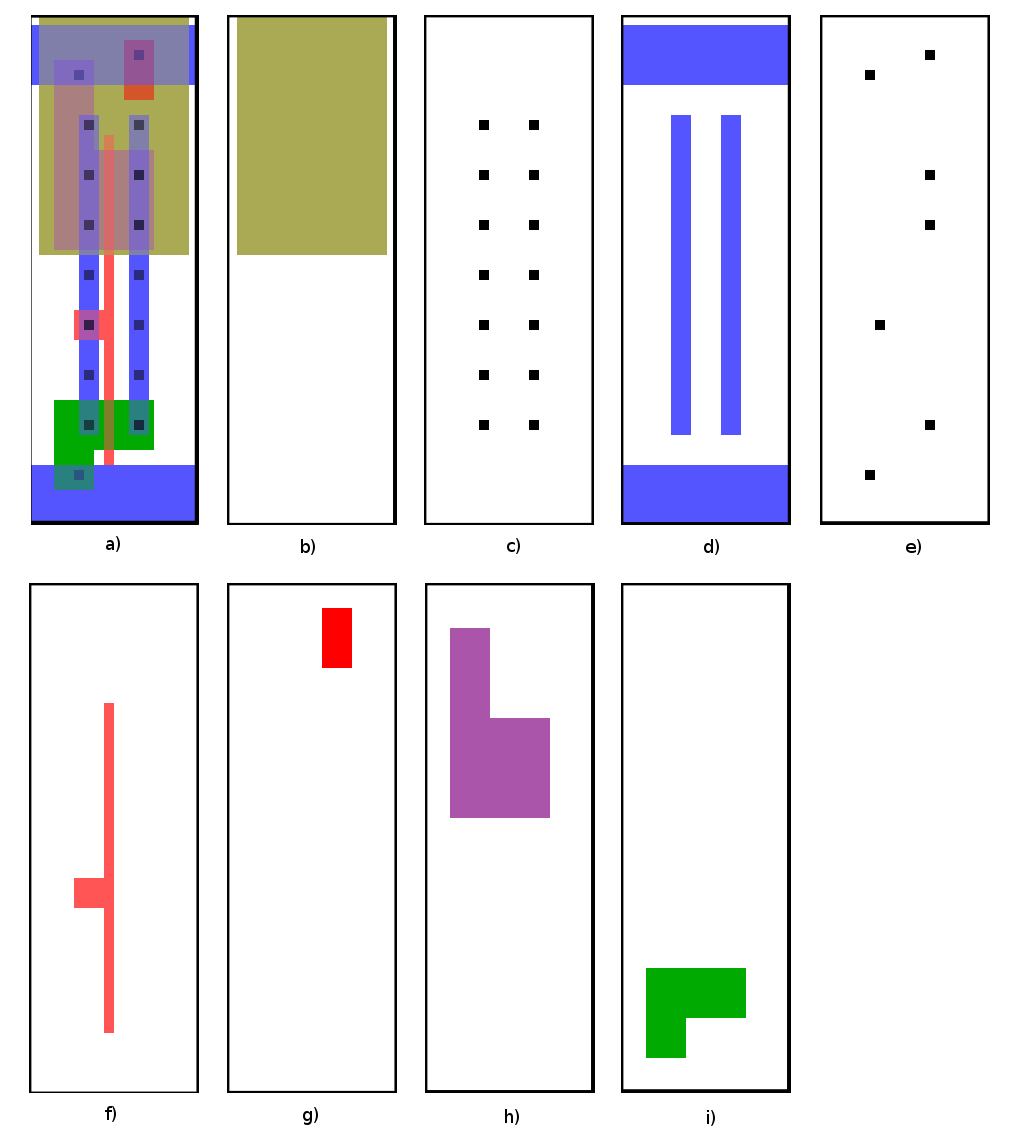
\includegraphics[scale=0.2, clip=true, trim= 0pt 0pt 0pt 0pt]{images/chapter03-image01}
	\caption{Basic inverter where all its layers has been separated: a) Full cell, b) NWELL, c) NDIF, d) PDIF, e) NTIE, f) POLY, g) CONT, h) ALU1, i) REF.}
\end{figure}

\subsection{Design coordinates}\label{Design-coordinates}

An Integrated Circuit design can be seen as a 2D area where all the components that form it are placed in a Cartesian Plane. In the figure \ref{fig:iccoordinates} can be seen such plane, in which can be found an origin (coordinates \texttt{[0,0]}), X increases to the right (and goes negative to the left) and Y increases to the top (and goes negative to the bottom). Most of the Integrated Circuit designs are defined and positioned in the first quadrant (positive values for the coordinates)\footnote{Is important to note that, even if most designs are defined in the first Cartesian quadrant, nothing prevents them to be defined in any of the other three quadrants.}, so the lower left corner of the design, usually, falls in the \texttt{[0,0]} coordinate of the plane.

\begin{figure}
	\centering
	\label{fig:iccoordinates}
	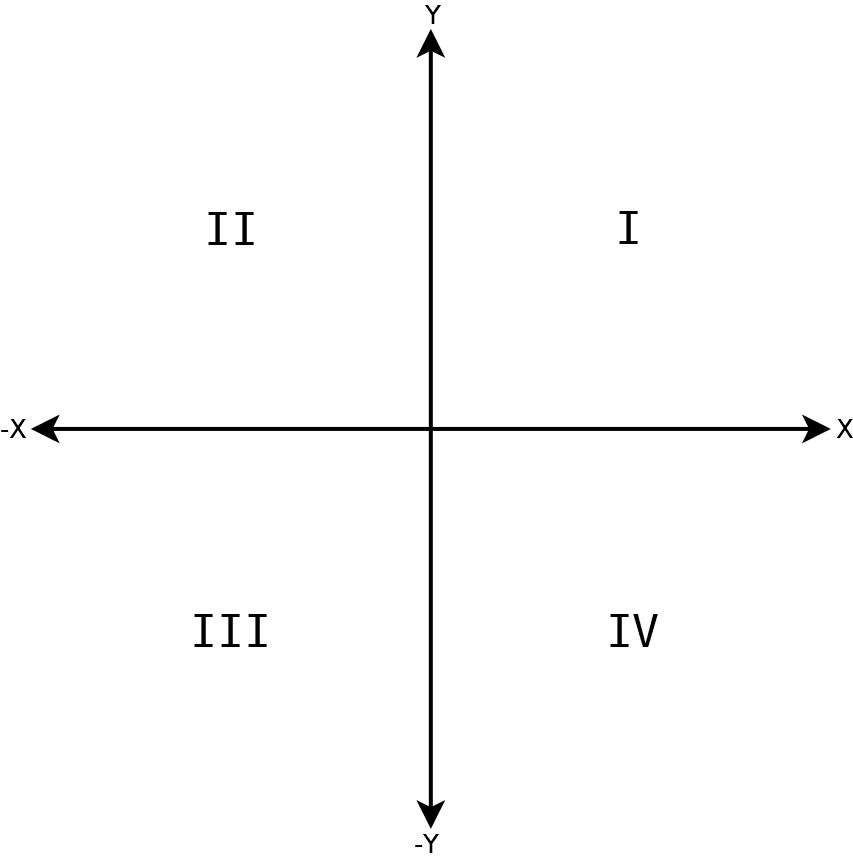
\includegraphics[scale=0.2, clip=true, trim= 0pt 0pt 0pt 0pt]{images/chapter03-image02}
	\caption{Representation of the Cartesian Plane used in the Integrated Designs.}
\end{figure}

Having the previous detail explained, is important to have in mind that the designs are intended to represent real components that are really small. Such components use as measuring unit the \textbf{micrometer} (\textbf{$\mu$}). This unit, even when it is really small, sometimes it not enough precision to represent coordinates nor sizes of pieces of the design, so, various components are measured in hundreds or even thousands of micrometer.

As can be seen, the precision of values is really important when working with Integrated Circuit designs. That brings the importance of floating point values and how to represent them in a design (and, more important, how to store them).

\subsection{Theorical and real precision of values}\label{Theorical-and-real-precision-of-values}

As previously mentioned, an Integrated Circuit design is composed by various geometrical figures. Those figures need to be placed with a high level of precision. The previous detail brings a great challenge to any format intended to store an Integrated Circuit design. Even beyond details of how to store the design structure, how to place components, how to correctly organize all the elements, the biggest problem to solve is precision. Various formats available (like the GDSII or OASIS) store the positions and sizes of components using floating point values in binary form, but such method has its limitations\footnote{However, in this document we will not touch other formats nor discuss if any is better than other, that is not the point of this document.} .

A floating point representation of a number in a design requires a nearly perfect representation of the original value. Such precision can be achieved using 32 bit floating point values, or even 64 bit floating point values, but even then, they have limitations about the length and real precision stored. Due to this complex problem of how to store a floating point value, the CIF format doesn't allow to use any value of such type. In a CIF file, all the values (positions and sizes) are stored as integer values, and if a floating point is required, an auxiliary \textbf{fraction} is used to scale the values (more of this later).

The idea behind the previously defined concept, is that the CIF format doesn't restrict the precision allowed to be used, so, all the tasks related to the process of loading and conversion of the values, are left to the applications that are intended to use the CIF files. Since the format itself doesn't restrict in any way the length (and therefore, the precision) of a value, all the applications that interact with CIF files must apply their own rules to be able to read such values and convert them, as precisely as possible, to floating point representations of the original values.

In a CIF file, even when using fractions to help represent high precision values, there is important to note that the values used in positions and sizes are, by themselves, \textbf{hundredths} of a \textbf{micrometer}. So, if a square is defined in a file as having a length of 100 units per side, we can say that such figure has a length of 1 $\mu$ per side. Also, as can be seen, this can be used to represent up to two decimal positions of a floating point value, this means that a value of 1234, in CIF format, represents a real value of 12.34 $\mu$.

With the previous details defined, we can start to define the basic components found in a design: The Primitive Commands.

\subsection{Primitive Commands}\label{Primitive-Commands}

The first group of commands, named in this document as \textbf{Primitive Commands}, are those that allow us to define, place and control geometrical figures. The figures that can be used are:

\begin{itemize}
\item Box
\item Polygon
\item Wire
\item Round Flash
\end{itemize}

A \textbf{Box} command defines a rectangle with some properties:

\begin{itemize}
\item Size
\item Position
\item Rotation
\end{itemize}

The \textbf{size} of a \textbf{Box} is defined as the \textbf{width} and \textbf{height} of such figure, and both values must be positive. The \textbf{position} of a \textbf{Box} is defined as the coordinates on which its \textbf{center} must be placed. The rotation of a Box is totally optional. The rotation is represented by the coordinates of a point. Such point, along with the center of the Box, forms an angle with respect of the X axis. Such angle is the rotation to be applied to the figure\footnote{If the Box has a rotation applied, it must rotate around its own center.} . There is important to note that all the rotations (no only for Boxes) are \textbf{counter-clockwise}, never \textbf{clockwise}. In the figure \ref{fig:boxrotation} can be seen an example, where a Box has a rotation described by the points [1,0], [1,1], [-1,-1] and [10,-1].

\begin{figure}
	\centering
	\label{fig:boxrotation}
	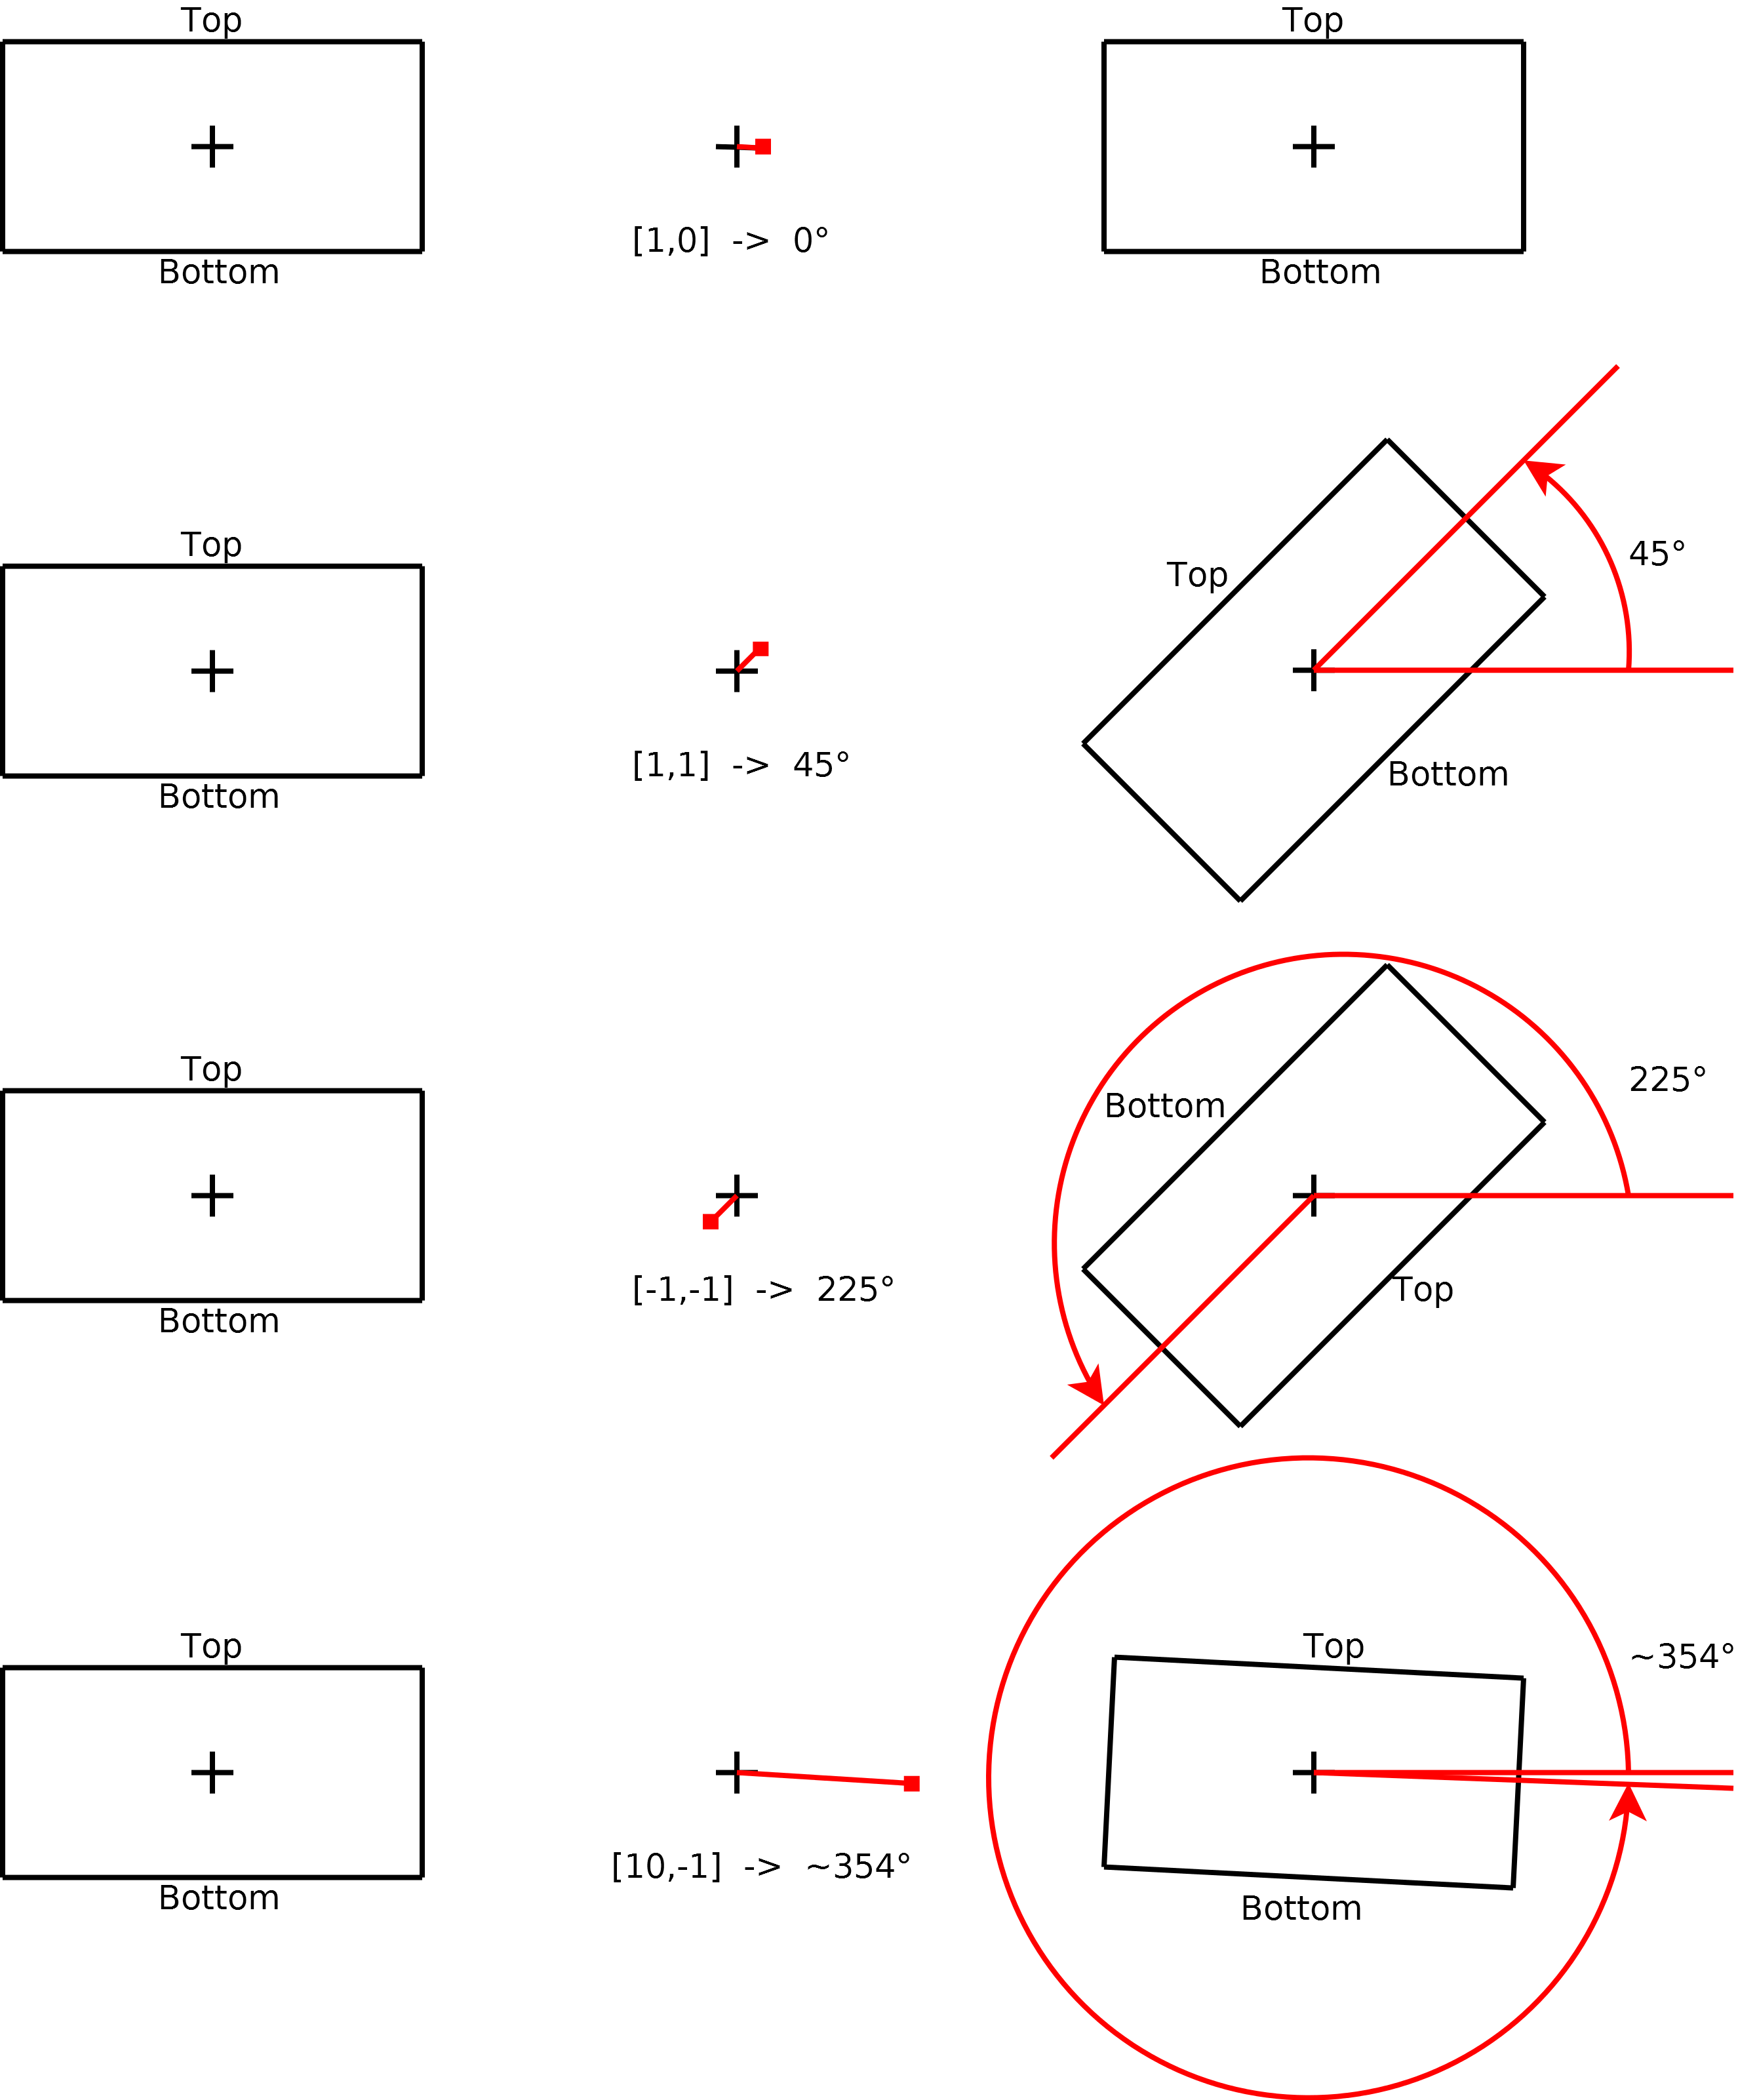
\includegraphics[scale=0.1, clip=true, trim= 0pt 0pt 0pt 0pt]{images/chapter03-image03}
	\caption{Visualization of the effect of the rotation over a Box object.}
\end{figure}

A \textbf{Polygon} defines a list of points that form a figure. Such figure can be as complex or simple as needed. The CIF format doesn't set any kind of restriction about which kind of figures can be defined. The polygons formed must be closed, so the first and last point are implicitly closed (there is no need that the first and last point be the same), can be concave and have self-interceptions. The figure \ref{fig:polygon} shows a basic example of a closed \textbf{Polygon}.

\begin{figure}
	\centering
	\label{fig:polygon}
	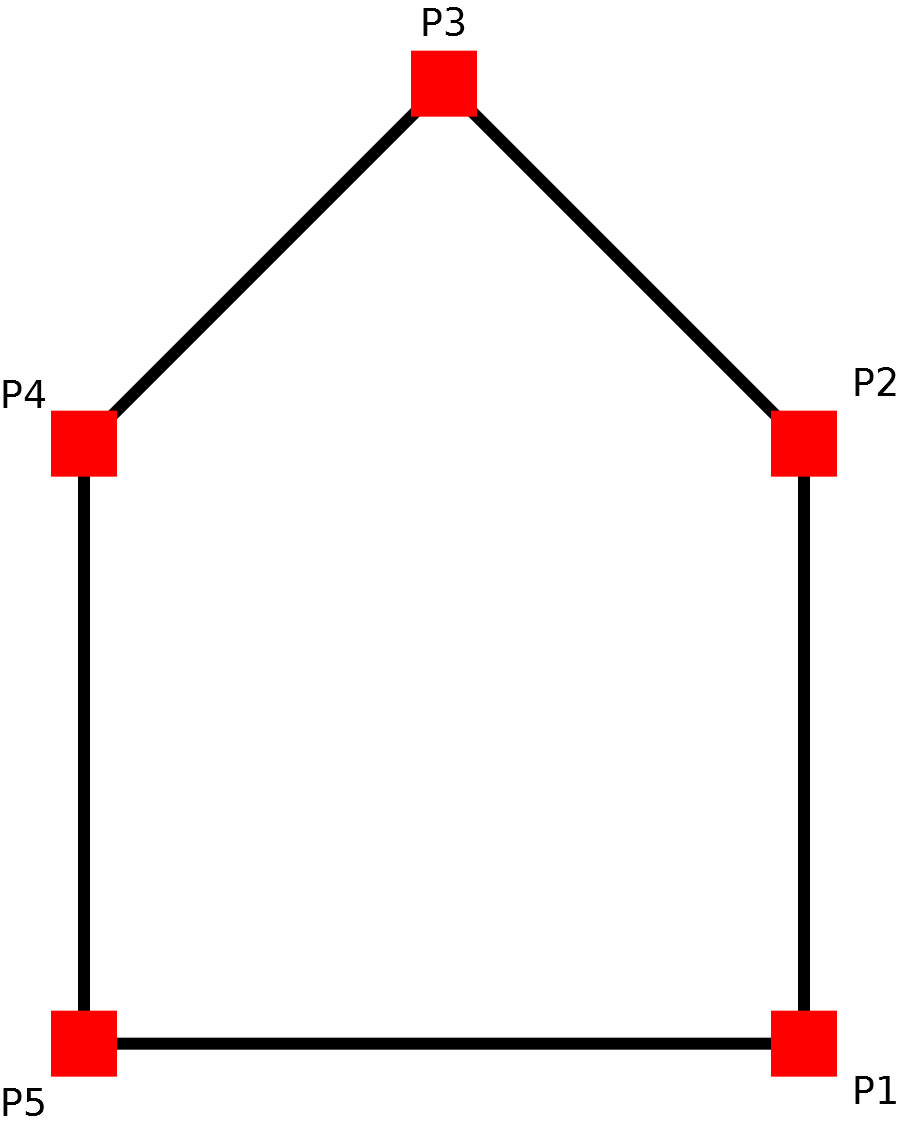
\includegraphics[scale=0.15, clip=true, trim= 0pt 0pt 0pt 0pt]{images/chapter03-image04}
	\caption{Visualization of an example of \textbf{Polygon}.}
\end{figure}

A \textbf{Wire} is similar to a \textbf{Polygon}. The \textbf{Wire} has the following properties:

\begin{itemize}
\item Width
\item List of points
\end{itemize}

The \textbf{Wire} defines a list of points that aren't a polygon, they're just a path of points over which a stripe of material will be placed, and the width defines the width of such stripe. The figure \ref{fig:polygon} shows a basic example of a \textbf{Wire} that has four points and a specific width.

\begin{figure}
	\centering
	\label{fig:wire}
	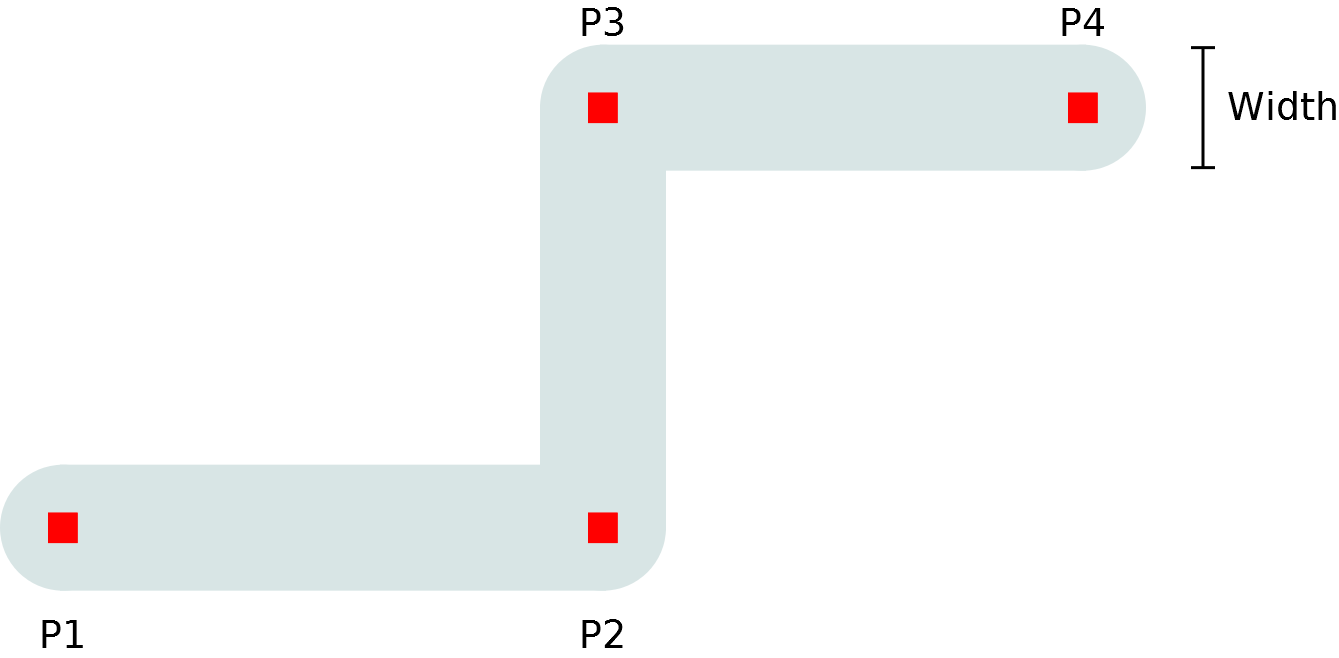
\includegraphics[scale=0.2, clip=true, trim= 0pt 0pt 0pt 0pt]{images/chapter03-image05}
	\caption{Visualization of an example of \textbf{Wire}.}
\end{figure}

The \textbf{Round Flash} defines a circle. Such figure has two properties:

\begin{itemize}
\item Position
\item Diameter
\end{itemize}

The \textbf{position} of a \textbf{Round Flash} corresponds to its center, while the \textbf{diameter} is its size. The figure \ref{fig:roundflash} shows a basic example of a \textbf{Round Flash}.

\begin{figure}
	\centering
	\label{fig:roundflash}
	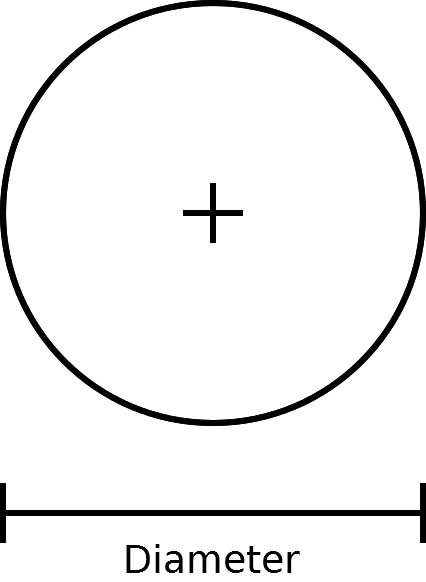
\includegraphics[scale=0.2, clip=true, trim= 0pt 0pt 0pt 0pt]{images/chapter03-image06}
	\caption{Visualization of an example of \textbf{Round Flash}.}
\end{figure}

The \textbf{Box} and \textbf{Polygon} figures are usually used to represent the smaller components that are used in an Integrated Circuit design and its power connections, while the \textbf{Wire} and \textbf{Round Flash} are usually used to form the data connection between  the small components.

\subsection{Control Commands}\label{Control-Commands}

The second group of commands, named in this document as \textbf{Control Commands}, are those that allow us to define, call, place and rotate those basic components of a design named \textbf{cells}.

The first element to understand is a low-level cell . Such component represent a small group of figures (Box, Polygon, Wire or Round Flash or the \textbf{Layer} and \textbf{User Extension} commands, discussed later). This kind of cell represents small mathematical operations, like an inverter, an OR or an AND, and can be used multiple times in a single Integrated Circuit design. To define such component we need two CIF commands. The first one defines a start and a second defines an end. All the commands found within this two commands are considered part of this cell. These two commands are known in this document as \textbf{Definition Start} and \textbf{Definition End}.

\IconNote
	{warning}
	{Cell or Symbol?}
	{In the CIF formal technical documentation, the cells are named \textbf{Symbols}, but most of the applications, books and almost any other documentation refers to the cells as \textbf{cells}. This detail must be handled with care. In this document, we refer to the cells as \textbf{cells}.}
	
The \textbf{Definition Start} command have two properties. The first is mandatory, and is an ID that must be assigned to the cell defined, so, that cell can be referred by its unique ID. The second is optional and is formed by two integers (named A and B) that defines a constant \textbf{fraction} for which will be multiplied all the size and position values inside the cell definition (this multiplication is used to convert big integers into small and precise floating point values).

The \textbf{Definition End} command doesn't need any properties, it just end the definition of a cell and must be preceded by a Definition Start command.

\IconNote
	{warning}
	{Cells within cells}
	{Is considered an error if a Definition Start command is found after another Definition Start command (before its closing Definition End is found).}
	
\IconNote
	{info}
	{Non-consecutive IDs}
	{The CIF format doesn't restrict in any way the order of the IDs used to define cells. They can have any integer as long as such value has not yet been used by another cell and it must be positive.}

The following command found in this group is a \textbf{Call} command. Such command is used to instantiate a previously defined cell. This behaves just like a function. The user can define small pieces of design (just like small pieces of code) and can use them whenever such component (of behaviour) is needed. As can be inferred, a cell can have calls to other cells that can, in turn, have calls to another cells, and so on.

\IconNote
	{warning}
	{Cycles are not good}
	{Even if in programming languages a function can be directly call himself, or indirectly call itself calling another function, in a CIF file, such call cycles are not possible and are considered an error since there is no code to stop such commands to call themselves infinitely.}
	
The \textbf{Call} command has two main group of properties. The first is mandatory and is the ID of the cell that must be called. Is important to note that such cell ID must be already defined when the Call command is found, in other case is considered an error. The second group of properties is a list of \textbf{Transformations} that can be applied to the cell called.

If no transformations are applied to the cell, the cell is just used as defined, so, for example, if there are three calls to the same cell, without any transformation, can be considered that there are three cells overlapped in the same position. Even if such situation is not an error \textit{per se}, is obvious that positioning the same components in the same position over and over is of no help for a design, so, most calls have at least one Transformation applied to the cell.

The transformations can be of three types: \textbf{Rotation}, \textbf{Translation} or \textbf{Mirror}.

A \textbf{Translation} transformation adds a very specific value to all the X and Y coordinates of all the elements found within a cell, so this transformation is used to call cells to a specific place in a design. The values used for this transformation are integers that can be positive or negative.

\IconNote
	{info}
	{Cell definitions}
	{Most of the times, the low-level cells are defined so their lower left corners are placed in the origin coordinates ([0,0]). This is done to simplify the process of calling cells in a design.}
	
A \textbf{Rotation} transformation, as can be inferred by its name, is used to rotate a cell with respect of the origin coordinates of the whole design. In a similar way as how a Box is rotated, a cell rotation is defined using two integers (that can be positive or negative) and represent the angle that the cell must be rotated. Also, as with the Box command, the rotation point can be arbitrary, so, any angle is allowed and it must be counter-clockwise.

A \textbf{Mirror} transformation is used to flip a design horizontally or vertically by multiplying the coordinates of the cell components by -1 in X or Y, depending on the transformation used\footnote{Is important to note that, for example, if a figure is located in the center of the first quadrant and an Mirror transformation is applied to it horizontally, the result must be it being placed, horizontally flipped and located in the \textbf{second quadrant} (such behaviour is not an error, is expected).}.

Another consideration with the transformations is that they no only apply to the figures defined within the cell called, they must be also applied to the Call commands found within this cell, so, they are applied recursively in the cell until no more Call commands are found. This is done to apply transformations no only to the top level cell, but to all the lower level cells.

The next command found in this group is the \textbf{Definition Delete} command. As far as the author experience can prove, this command is not extensively used in the Integrated Circuit designs. It is used to remove a previously defined cell, so its ID is available to use again and its contents are not available. This command is useful if the CIF file is being processed command by command (in a linear way) so that cells that are not going to be used again in the design can be safety deleted (freeing memory from the reading device or program). Even if this command is not widely used in today designs, the support must be provided.

The Definition Delete command has one mandatory property, and it is the ID of the cell (that must be already defined) to delete. When deleting, is expected to delete only the direct contents of the cell referred, not the cells mentioned in call commands found within the deleted cell.

The last command found in this group is the \textbf{End} command. Such command is intended to mark the \textbf{end of the file}. Even if the file has contents later, if this command is found, the reading application or device must consider that the design is over.

\subsection{RAW content commands}\label{RAW-content-commands}

This group of commands include those which contents are user-defined and that doesn't require any validation from the reading application or device. Any interpretation performed over the contents of these commands are directly dependant of the reading application or device, so, are not covered by the format itself and might not be compatible between applications.

The first command found in this group is the \textbf{User Extension} command. This command is intended to provide a way to extend the functionality and capabilities of the format, allowing to define new commands that are application dependant. These commands allow, in some common situations, to define the name of cells and to define connection points, port names and other details that are equally important in a design, but that the CIF format, \textit{per se}, doesn't allow to define.

The second and last command of this group is the \textbf{Comment} command. These commands are intended to introduce comment lines on a design to store information not directly used in the design, like author name, date on which the design was stored, or a description of the design.

\subsection{Layer command}\label{Layer-command}

An Integrated Circuit design is composed, as discussed, by geometrical figures that represent components of a design. Those figures must be made of some material and such material must be defined. In a CIF file, exist the \textbf{Layer} command, that allow the reader application to know of which material are made the figures it is reading.

When reading a CIF file, once the user finds a Layer command, the following Primitive Commands that it finds can be considered to be made of the material specified by the previously found Layer command. To change the material of which a figure is made, a new Layer command must be placed. As can be seen, all the Primitive commands found after a Layer command are made of the material specified unless a new Layer command is found.

The Layer command has one mandatory property. Such property is the name of the material to use. The initial definition of this command states that the name must be formed with 4 characters, but, since various applications using the CIF format doesn't respect this restriction (using names shorter or longer than 4 characters), this library, when validating a CIF file, will not have in consideration the length of the material names\footnote{Is also important to note that most applications use their own set of material names even if there exist a standard that respects the 4-char rule.}.

\subsection{BNF representation of the format}\label{BNF-representation-of-the-format}

All the components that form an Integrated Circuit design can be represented by the CIF format using the supported \textbf{commands} that where previously described. The CIF commands need to be represented and identified using as less characters as possible. So, the solution used by the format is to represent every command with a specific character. The following text defines the complete \textbf{BNF} (Backus Naur Form) description of the format\footnote{The format described in this document is not exactly the same as that described in the official documentation. The \textbf{BNF} description is adapted to the purposes of this document.}. The BNF is described using the following rules:

\begin{itemize}
\item The curly brackets represent a repetition of one or more of its contents.
\item The brackets represents that its contents are optional (can or can't be present).
\item A character within apostrophes means that it is a literal character.
\item The parentheses represent selection between its contents (separated by pipes).
\end{itemize}

\begin{verbatim}
FILE ::= {COMMAND}
BLANK ::= Any ASCII except DIGIT, UPPER, '-', '(', ')' or ';'
DIGIT ::= Any digit from '0' to '9'
UPPER ::= Any character from 'A' to 'Z'
SEP ::= An UPPER or BLANK
POINT ::= ['-'] {DIGIT} {SEP} ['-'] {DIGIT}
INTEGER ::= {DIGIT}
LAYERCHAR ::= A DIGIT, UPPER or '_'
EXTCHAR ::= Any ASCII character except ';'
COMMENTCHAR ::= Any ASCII character except '(' or ')'
COMMAND ::= [{BLANK}] ( PRIMITIVE | CONTROL | EXTENSION | COMMENT )
PRIMITIVE ::= ( POLYGON | BOX | ROUNDFLASH | WIRE )
CONTROL ::= ( LAYER | SYMSTART | SYMEND | SYMDEL | CALL | END )
POLYGON ::= 'P' [{BLANK}] POINT [{SEP POINT}] [{SEP}] ';'
BOX ::= 'B' [{BLANK}] INTEGER {SEP} INTEGER {SEP} POINT [ {SEP} POINT [{SEP}] ] ';'
ROUNDFLASH ::= 'R' [{BLANK}] INTEGER {SEP} POINT [{SEP}] ';'
WIRE ::= 'W' [{BLANK}] INTEGER {SEP} POINT [{SEP POINT}] [{SEP}] ';'
LAYER ::= 'L' [{BLANK}] {LAYERCHAR} [{BLANK}] ';'
SYMSTART ::= 'D' [{BLANK}]'S' [{SEP}] INTEGER [{SEP}INTEGER{SEP} INTEGER] [{SEP}] ';'
SYMEND ::= 'D' [{BLANK}] 'F' [{SEP}] ';'
SYMDEL ::= 'D' [{BLANK}] 'D' [{BLANK}] INTEGER [{SEP}] ';'
CALL ::= 'C' [{BLANK}] INTEGER [{[{BLANK}] (TRANS | MIRROR | ROTATION)}] [{BLANK}] ';'
TRANS ::= 'T' [{BLANK}] POINT
MIRROR ::= 'M' [{BLANK}] ('X' | 'Y')
ROTATION ::= 'R' [{BLANK}] POINT
EXTENTION ::= DIGIT [{EXTCHAR}] ';'
COMMENT ::= '(' [{COMMENTCHAR}] ')' [{BLANK}] ';'
END ::= 'E' [ [{SEP}] ';' ]
\end{verbatim}

The previous definition explains, in BNF format, how a CIF file is structured. Some of the differences between the definition presented and the official definition are these:

\begin{itemize}
\item The order on which the format defines how components (specially the whitespaces) are used is different in order to try to prevent a non-deterministic definition.
\item Since in the real world exists examples of production designs that doesn't respect the 4-character rule for the layer names, in our format we are not limiting the names to those 4 characters.
\item The format doesn't have in consideration the possible contents of the file beyond the END command since such contents are not of interest for the design (but are not considered an error \textit{per se}).
\item There must not be considered a non-deterministic problem the definition of the SEP character. The uppercase characters (A to Z) must override the definition of the BLANK character.
\end{itemize}

\IconNote
	{info}
	{Validating two points of view}
	{Is recommended for the user to take a look at the original documentation to compare our definition and the original one.}

As can be seen, there is important to note that the CIF format defines that all the commands need to end using a semicolon\footnote{In the End command, the semicolon is optional but recommended.} and that most of the commands can be identified by their first character (an upper case character or a digit in the Expansion command).

After defining the contents of a CIF file, the next step is to understand how this library is able to load and validate the commands found in it.

%%%%%%%%%%%%%%%%%%%%%%%%%%%%%%%%%%%%%%%%%%%%%%%%%%%%%%%%%%%%%%%%%%
\section{Validation of a CIF file}\label{Validation-of-a-cif-file}
%%%%%%%%%%%%%%%%%%%%%%%%%%%%%%%%%%%%%%%%%%%%%%%%%%%%%%%%%%%%%%%%%%

This library has the purpose of loading into memory the contents of a CIF file. Such operation requires a validation of the contents loaded to be sure that they are correct and that they meet the format considered. The validation is performed loading the CIF file byte by byte and passing each one into a \textbf{Finite State Machine} which is designed to validate the possible structure of the CIF file.

The basic idea of the loading and validation process can be seen in the figure \ref{fig:basicloading}.

\begin{figure}
	\centering
	\label{fig:basicloading}
	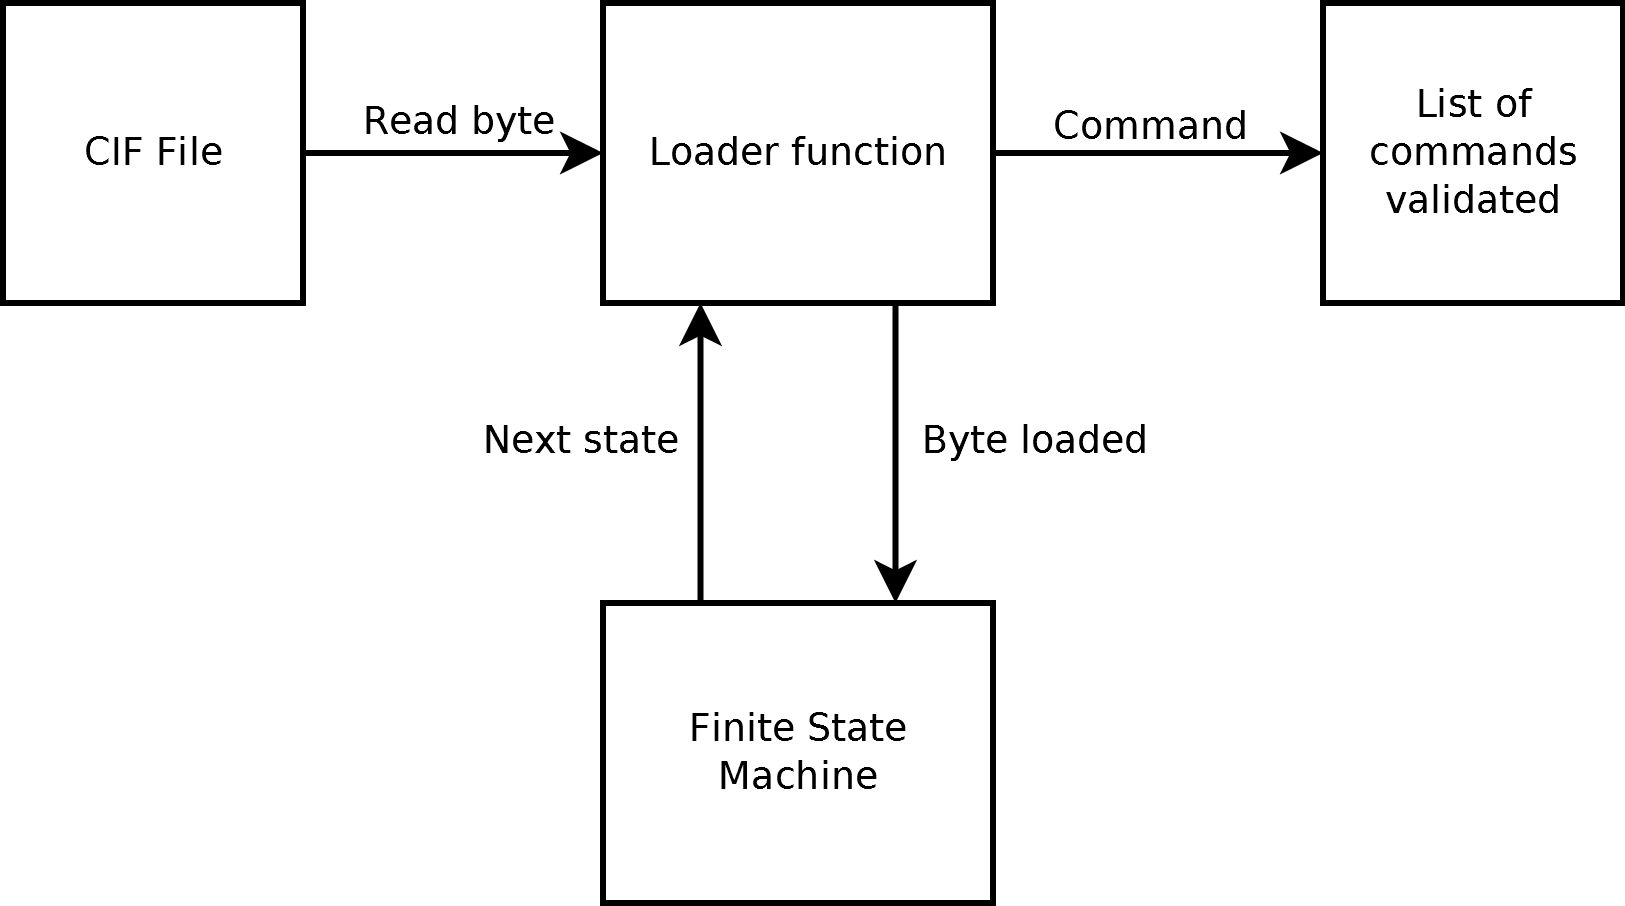
\includegraphics[scale=0.2, clip=true, trim= 0pt 0pt 0pt 0pt]{images/chapter03-image07}
	\caption{Basic diagram of the loading process of a CIF file by this library.}
\end{figure}

The loading is performed reading one byte from the file and sending such byte to the Finite State Machine, which, in turn, having control of the current state, validates the transition needed, returning the new state to the loading function. The loading function, in turn, validates the state returned by the Finite State Machine. If the state is not an Error State, then the byte is correct. Also, the loading function validates if the returned state means that the loaded byte completed a valid command (which was being stored in a buffer). If such situation is reached, the command is moved to the list of valid commands and the buffer is cleared.

Such process is repeated until the end of the file is reached, the End command is found or an error is detected.

%%%%%%%%%%%%%%%%%%%%%%%%%%%%%%%%%%%%%%%%%%%%%%%%%%%%%%%%%%%%%%%%%%%%%%%
\subsection{Finite state machine used}\label{Finite-state-machine-used}
%%%%%%%%%%%%%%%%%%%%%%%%%%%%%%%%%%%%%%%%%%%%%%%%%%%%%%%%%%%%%%%%%%%%%%%

Even more important that the process of how to read a byte from a file, the truly crucial detail, when validating a file using a Finite State Machine, is how such Finite State Machine is designed. In this case, the design was carefully made, trying to include as much information as possible.

The diagram of such design is too big for this document, so, the image must be available alongside this document.

The first thing the user will be able to see is a little indication of how to interpret the connections between states in the diagram (see figure \ref{fig:fsmconnections}).

\begin{figure}
	\centering
	\label{fig:fsmconnections}
	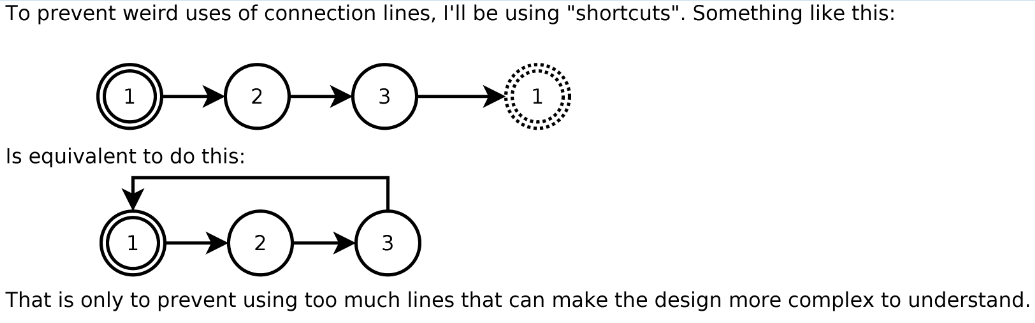
\includegraphics[scale=0.5, clip=true, trim= 0pt 0pt 0pt 0pt]{images/chapter03-image08}
	\caption{Basic diagram of the loading process of a CIF file by this library.}
\end{figure}

After that, comes a little section intended to understand the different groups of characters considered:

\begin{description}
\item[D]	Digits, characters from '0' to '9'.
\item[U]	Uppercase characters, from 'A' to 'Z'.
\item[B]	Blank characters, any ASCII character except digits, uppercase, minus (-), parentheses or semicolon.
\item[C]	Comment characters, any ASCII character except parentheses.
\item[S]	Separator characters, an uppercase character or Blank.
\item[L]	Layer name characters, any digit, uppercase character or '\_' character.
\end{description}

After checking the diagram, the user can see three terminal states: 1, 91 and 92. The state 1 is the starting point of the diagram. Such state is in charge of skipping Blank characters (characters found between commands that are of no use for the design). Every row represents a possible command. All of them start in the state 1 when it detects the starting character of one of it. All the commands end with semicolon. The End command is special, it doesn't need to end with semicolon (state 91) or, after finding it, is just matter of skipping characters (state 92) until the end of the file.

%%%%%%%%%%%%%%%%%%%%%%%%%%%%%%%%%%%%%%%%%%%%%%%%%
\subsection{Considerations}\label{Considerations}
%%%%%%%%%%%%%%%%%%%%%%%%%%%%%%%%%%%%%%%%%%%%%%%%%

There are some considerations that must be keep in mind at all times, because without them, the diagram can be considered to have flaws:

\begin{enumerate}
\item The comment command (state 89) isn't considering the fact that most applications support that a comment have internal parentheses. That is, that, meanwhile the parentheses are all closed before the comment command truly ends, there is no problem. That problem is solved in the implementation using some simple counters to know how many parentheses are left to close.
\end{enumerate}

%%%%%%%%%%%%%%%%%%%%%%%%%%%%%%%%%%%%%%%%%%%%%%%%%%%%%%%%%%%%
\section{Loading of a CIF file}\label{Loading-of-a-CIF-file}
%%%%%%%%%%%%%%%%%%%%%%%%%%%%%%%%%%%%%%%%%%%%%%%%%%%%%%%%%%%%

The loading of a CIF file, as considered, requires some options to be available to the user. One of such options is the process of loading a CIF file into memory and make the commands available to the user in string form and in class instance form. This design decision is intented to make the life of the user more easy, providing it with the required elements so the results can be used as needed.

%%%%%%%%%%%%%%%%%%%%%%%%%%%%%%%%%%%%%%%%%%%%%%%%%%%%%%%%%%%%%%%%%%%%%%%%%%%%%
\subsection{Cleaning process of commands}\label{Cleaning-process-of-commands}
%%%%%%%%%%%%%%%%%%%%%%%%%%%%%%%%%%%%%%%%%%%%%%%%%%%%%%%%%%%%%%%%%%%%%%%%%%%%%

One of the major options provided to the user is the cleaning of the commands. Even if the library can provide to the user the raw (but validated) commands, they can be hard to process because the extra characters that can be found. So, one of the biggest implementations done is the cleaning process. Such option was partitioned according to small groups of commands that can be cleaned in the same way.

%%%%%%%%%%%%%%%%%%%%%%%%%%%%%%%%%%%%%%%%%%%%%%%%%%%%%%%%
\subsubsection{Numeric commands}\label{Numeric-commands}
%%%%%%%%%%%%%%%%%%%%%%%%%%%%%%%%%%%%%%%%%%%%%%%%%%%%%%%%

The numeric commands are those that only contain their identification character and, after that, just numeric values. The commands considered to be numeric are:

\begin{itemize}
\item Polygon
\item Box
\item Wire
\item RoundFlash
\end{itemize}

These commands can be cleaned in the same way. The basic operation is very easy to implement. The first step is to backup the identification character and assign it to a new empty string with a whitespace after it. The second step is to iterate over the characters of the command and replace all the characters that are not digits or minus ('-') with whitespaces. This process will remove any not required character from the string, leaving only the good ones. Since the command string was already validated by the Finite State Machine, we can safely assume that all the remaining characters are always command characters.

The following string is an example of a "dirty" command:

\begin{verbatim}
W1000lol20000,,,this,is,valid20000xoxoxoxoxox-10000,-10000,-500example-4000;
\end{verbatim}

And so, the result of this first step is the following string:

\begin{verbatim}
 1000   20000                20000            -10000 -10000 -500       -4000
\end{verbatim}

Now, as can be seen, the command might be cleaner, but it still has lots of whitespaces and it doesn't have a semicolon. The idea is to convert it into the following string:

\begin{verbatim}
W 1000 20000 20000 -10000 -10000 -500 -4000 ;
\end{verbatim}

The goal is to remove all the whitespaces and add one after the identification character and before the semicolon. Using the previously created string (that contains the identification character and a whitespace), we will start concatenating to it the remaining pieces of command (separated by single whitespaces). To do such operation, we start with a \textit{istringstream} class instance. We create it with the partially cleaned command as constructor argument.

Using the previously created instance, we start to iterate over the process of extracting a word (a string) from the instance, until we reach the End Of File of such stream. Each word extracted will be contactenated to the temporal string (the one that has the identification character), with a trailing whitespace.

After this loop, we just need to concatenate the final semicolon with a trailing whitespace.

The last step on the cleaning process is to return the newly formed string to the caller.

%%%%%%%%%%%%%%%%%%%%%%%%%%%%%%%%%%%%%%%%%%%%%%%%%%%%
\subsubsection{Layer commands}\label{Layer-commands}
%%%%%%%%%%%%%%%%%%%%%%%%%%%%%%%%%%%%%%%%%%%%%%%%%%%%

The Layer commands are those that only contain their identification character and, after that, only uppercase characters, underscores and digits.

The basic operation is very easy to implement. The first step is to backup the identification character and assign it to a new empty string with a whitespace after it. Then, we manually replace the first character with a whitespace. The third step is to iterate over the characters of the command and replace all the characters that are not digits, uppercase characters or underscores with whitespaces. This process will remove any not required character from the string, leaving only the good ones. Since the command string was already validated by the Finite State Machine, we can safely assume that all the remaining characters are always command characters.

The following string is an example of a "dirty" command:

\begin{verbatim}
Lthis.is,,and.examplePOLY_OTHERx;
\end{verbatim}

And so, the result of this first step is the following string:

\begin{verbatim}
                     POLY_OTHER  
\end{verbatim}

Now, as can be seen, the command might be cleaner, but it still has lots of whitespaces and it doesn't have a semicolon. The idea is to convert it into the following string:

\begin{verbatim}
L POLY_OTHER ;
\end{verbatim}

The goal is to remove all the whitespaces and add one after the identification character and before the semicolon. Using the previously created string (that contains the identification character and a whitespace), we will start concatenating to it the remaining pieces of command (separated by single whitespaces). To do such operation, we start with a \textit{istringstream} class instance. We create it with the partially cleaned command as constructor argument.

Using the previously created instance, we start to iterate over the process of extracting a word (a string) from the instance, until we reach the End Of File of such stream. Each word extracted will be contactenated to the temporal string (the one that has the identification character), with a trailing whitespace.

After this loop, we just need to concatenate the final semicolon with a trailing whitespace.

The last step on the cleaning process is to return the newly formed string to the caller.

\IconNote
	{info}
	{Multiple words in a layer name}
	{The CIF format doesn't allow layer names to contain spaces (so, "POLY METAL" is invalid). The idea of using a istringstream isn't invalid since the command was already validated by the Finite State Machine, and is guaranteed that it has only one word.}

%%%%%%%%%%%%%%%%%%%%%%%%%%%%%%%%%%%%%%%%%%%%%%%%%%
\subsubsection{Call commands}\label{Call-commands}
%%%%%%%%%%%%%%%%%%%%%%%%%%%%%%%%%%%%%%%%%%%%%%%%%%

The Call commands are those that only contain their identification character and, after that, only uppercase characters and digits.

The basic operation is very easy to implement. The first step is to backup the identification character and assign it to a new empty string with a whitespace after it. Then, we manually replace the first character with a whitespace. The third step is to iterate over the characters of the command and replace all the characters that are not digits, uppercase characters or minus with whitespaces. This process will remove any not required character from the string, leaving only the good ones. Since the command string was already validated by the Finite State Machine, we can safely assume that all the remaining characters are always command characters.

The following string is an example of a "dirty" command:

\begin{verbatim}
C1T20000 -20000R1000000 -59999MXexampleMY MXMXMXMYMXR100 100R100 100;
\end{verbatim}

And so, the result of this first step is the following string:

\begin{verbatim}
 1T20000 -20000R1000000 -59999MX       MY MXMXMXMYMXR100 100R100 100 
\end{verbatim}

Now, as can be seen, the command might be cleaner, but it still has lots of whitespaces and other components of the command (like the Mirror options) are just too close (we need more whitespaces), and also it doesn't have a semicolon. The idea is to convert it into the following string:

\begin{verbatim}
C 1 T 20000 -20000 R 1000000 -59999 M X M Y M X M X M X M Y M X R 100 100 R 100 100 ;
\end{verbatim}

The goal is to remove all the whitespaces and add one after the identification character, before the semicolon and between the call options. Now, the cleaning process of this step is a little bit more complicated that the previousn ones. In this case, we need to split a string without clear indications of wherer we need to cut. To process the string, we will use some properties of the command format:

\begin{enumerate}
\item The numbers found in the command can't be togheter, that is, that between each one must be a whitespace or an uppercase character.
\item There can't be two whitespaces togheter. If two or more whitespaces are found, we will remove all but the first.
\item The uppercase characters (the call options) require to have whitespaces before and after them.
\item The minus character requires a whitespace before it.
\end{enumerate}

The previously defined properties can be used to define a code block that is able to process the whole command, adding the required whitespaces and removing the extra ones:

\lstinputlisting[caption={Implemented block of code using the properties of the Call Command.}, style=CPPStyle]{examples/chapter3-example3.cc}

Using the previous code block, we can correctly format the contents of the Call Command. After this loop, we just need to concatenate the final semicolon with a trailing whitespace.

The last step on the cleaning process is to return the newly formed string to the caller.

%%%%%%%%%%%%%%%%%%%%%%%%%%%%%%%%%%%%%%%%%%%%%%%%%%%%%%%%%%%%%%%%%%%%%%%%%%%%%%
\subsubsection{Definition control commands}\label{Definition-control-commands}
%%%%%%%%%%%%%%%%%%%%%%%%%%%%%%%%%%%%%%%%%%%%%%%%%%%%%%%%%%%%%%%%%%%%%%%%%%%%%%

The Definition control commands are those that contain their identification characters and, after that, only digits.

The basic operation is very easy to implement. The first step is to backup the first identification character and assign it to a new empty string with a whitespace after it. Then, we manually replace the first character with a whitespace. The third step is to iterate over the characters of the command and replace all the characters that are not digits or uppercase characters. This process will remove any not required character from the string, leaving only the good ones. Since the command string was already validated by the Finite State Machine, we can safely assume that all the remaining characters are always command characters.

The following string is an example of a "dirty" command:

\begin{verbatim}
DxxxxxSlol100im,totally,correct;
\end{verbatim}

And so, the result of this first step is the following string:

\begin{verbatim}
      S   100                   
\end{verbatim}

Now, as can be seen, the command might be cleaner, but it still has lots of whitespaces and it doesn't have a semicolon. The idea is to convert it into the following string:

\begin{verbatim}
D S 100 ;
\end{verbatim}

The goal is to remove all the whitespaces and add one after the identification character, before the semicolon and between the call options. Now, the cleaning process of this step is a little bit more complicated that the previousn ones (but similar to the one found for the Call Command, just a little bit more simple). In this case, we need to split a string without clear indications of wherer we need to cut. To process the string, we will use some properties of the command format:

\begin{enumerate}
\item The numbers found in the command can't be togheter, that is, that between each one must be a whitespace or an uppercase character.
\item There can't be two whitespaces togheter. If two or more whitespaces are found, we will remove all but the first.
\item The uppercase characters (the second identification character) require to have whitespaces before and after them.
\end{enumerate}

The previously defined properties can be used to define a code block that is able to process the whole command, adding the required whitespaces and removing the extra ones:

\lstinputlisting[caption={Implemented block of code using the properties of the Call Command.}, style=CPPStyle]{examples/chapter3-example4.cc}

Using the previous code block, we can correctly format the contents of the Definition Commands. After this loop, we just need to concatenate the final semicolon with a trailing whitespace.

The last step on the cleaning process is to return the newly formed string to the caller.

%%%%%%%%%%%%%%%%%%%%%%%%%%%%%%%%%%%%%%%%%%%%%%%%%%%%%%%%%%%%%%%%%%%%%%%%%%%%%%
\subsubsection{Expansion commands}\label{Expansion-commands}
%%%%%%%%%%%%%%%%%%%%%%%%%%%%%%%%%%%%%%%%%%%%%%%%%%%%%%%%%%%%%%%%%%%%%%%%%%%%%%

The Expansion commands are those that contain their identification characters and, after that, any character that the user might require.

These commands are the easiest to process, since they only require to have their identification charcters separated. The followin is an example of valid command:

\begin{verbatim}
9 CORE;
\end{verbatim}

In this example, the Expansion command ID is "9", and its content "CORE" must be processed and validated by the application loading the file. The CIF format itself doesn't give any special meaning to the Expansion commands, so, in this library they are being as they are defined.

%%%%%%%%%%%%%%%%%%%%%%%%%%%%%%%%%%%%%%%%%%%%%%%%%
\section{Converting strings into class instances}\label{Converting-strings-into-class-instances}
%%%%%%%%%%%%%%%%%%%%%%%%%%%%%%%%%%%%%%%%%%%%%%%%%

In this last section of the document, the user will learn about the design of the classes that can be found within the library. Once the commands are totally validated and cleaned, they can be converted into class instances to be used by the user as needed.

%%%%%%%%%%%%%%%%%%%%%%%%%%%%%%%%%%%%%%%%%%%%%%%%%%%%%%%%%%%%%%%%%%%%%%%%%%%
\subsection{Validation group of classes}\label{Validation-group-of-classes}
%%%%%%%%%%%%%%%%%%%%%%%%%%%%%%%%%%%%%%%%%%%%%%%%%%%%%%%%%%%%%%%%%%%%%%%%%%%

Validation group of classes

%%%%%%%%%%%%%%%%%%%%%%%%%%%%%%%%%%%%%%%%%%%%%%%
\subsubsection{Class: State}\label{Class-State}
%%%%%%%%%%%%%%%%%%%%%%%%%%%%%%%%%%%%%%%%%%%%%%%

Class: State

%%%%%%%%%%%%%%%%%%%%%%%%%%%%%%%%%%%%%%%%%%%%%%%%%%%%%%%%%%%%%%%%%%%%%%%%%
\subsubsection{Class: FiniteStateMachine}\label{Class-FiniteStateMachine}
%%%%%%%%%%%%%%%%%%%%%%%%%%%%%%%%%%%%%%%%%%%%%%%%%%%%%%%%%%%%%%%%%%%%%%%%%

Class: FiniteStateMachine

%%%%%%%%%%%%%%%%%%%%%%%%%%%%%%%%%%%%%%%%%%%%%%%%%
\subsubsection{Class: CIFFSM}\label{Class-CIFFSM}
%%%%%%%%%%%%%%%%%%%%%%%%%%%%%%%%%%%%%%%%%%%%%%%%%

Class: CIFFSM

%%%%%%%%%%%%%%%%%%%%%%%%%%%%%%%%%%%%%%%%%%%%%%%%%%%%%%%%%%%%%%%%%%%%%
\subsection{Command group of classes}\label{Command-group-of-classes}
%%%%%%%%%%%%%%%%%%%%%%%%%%%%%%%%%%%%%%%%%%%%%%%%%%%%%%%%%%%%%%%%%%%%%

Command group of classes

%%%%%%%%%%%%%%%%%%%%%%%%%%%%%%%%%%%%%%%%%%%%%%%
\subsubsection{Class: Point}\label{Class-Point}
%%%%%%%%%%%%%%%%%%%%%%%%%%%%%%%%%%%%%%%%%%%%%%%

Class: Point

%%%%%%%%%%%%%%%%%%%%%%%%%%%%%%%%%%%%%%%%%%%%%
\subsubsection{Class: Size}\label{Class-Size}
%%%%%%%%%%%%%%%%%%%%%%%%%%%%%%%%%%%%%%%%%%%%%

Class: Size

%%%%%%%%%%%%%%%%%%%%%%%%%%%%%%%%%%%%%%%%%%%%%%%%%%%%%
\subsubsection{Class: Fraction}\label{Class-Fraction}
%%%%%%%%%%%%%%%%%%%%%%%%%%%%%%%%%%%%%%%%%%%%%%%%%%%%%

Class: Fraction

%%%%%%%%%%%%%%%%%%%%%%%%%%%%%%%%%%%%%%%%%%%%%%%%%%%%%%%%%%%%%%%%%
\subsubsection{Class: Transformation}\label{Class-Transformation}
%%%%%%%%%%%%%%%%%%%%%%%%%%%%%%%%%%%%%%%%%%%%%%%%%%%%%%%%%%%%%%%%%

Class: Transformation

%%%%%%%%%%%%%%%%%%%%%%%%%%%%%%%%%%%%%%%%%%%%%%%%%%%
\subsubsection{Class: Command}\label{Class-Command}
%%%%%%%%%%%%%%%%%%%%%%%%%%%%%%%%%%%%%%%%%%%%%%%%%%%

Class: Command

%%%%%%%%%%%%%%%%%%%%%%%%%%%%%%%%%%%%%%%%%%%%%%%%%%%%%%%%%%%%%%%%%%%%%
\subsubsection{Class: PrimitiveCommand}\label{Class-PrimitiveCommand}
%%%%%%%%%%%%%%%%%%%%%%%%%%%%%%%%%%%%%%%%%%%%%%%%%%%%%%%%%%%%%%%%%%%%%

Class: PrimitiveCommand

%%%%%%%%%%%%%%%%%%%%%%%%%%%%%%%%%%%%%%%%%%%%%%%%%%%%%%%%%%%%%%%%%%%%%
\subsubsection{Class: PathBasedCommand}\label{Class-PathBasedCommand}
%%%%%%%%%%%%%%%%%%%%%%%%%%%%%%%%%%%%%%%%%%%%%%%%%%%%%%%%%%%%%%%%%%%%%

Class: PathBasedCommand

%%%%%%%%%%%%%%%%%%%%%%%%%%%%%%%%%%%%%%%%%%%%%%%%%%%%%%%%%%%%%%%%%
\subsubsection{Class: PolygonCommand}\label{Class-PolygonCommand}
%%%%%%%%%%%%%%%%%%%%%%%%%%%%%%%%%%%%%%%%%%%%%%%%%%%%%%%%%%%%%%%%%

Class: PolygonCommand

%%%%%%%%%%%%%%%%%%%%%%%%%%%%%%%%%%%%%%%%%%%%%%%%%%%%%%%%%%%
\subsubsection{Class: WireCommand}\label{Class-WireCommand}
%%%%%%%%%%%%%%%%%%%%%%%%%%%%%%%%%%%%%%%%%%%%%%%%%%%%%%%%%%%

Class: WireCommand

%%%%%%%%%%%%%%%%%%%%%%%%%%%%%%%%%%%%%%%%%%%%%%%%%%%%%%%%%%%%%%%%%%%%%%%%%%%%%
\subsubsection{Class: PositionBasedCommand}\label{Class-PositionBasedCommand}
%%%%%%%%%%%%%%%%%%%%%%%%%%%%%%%%%%%%%%%%%%%%%%%%%%%%%%%%%%%%%%%%%%%%%%%%%%%%%

Class: PositionBasedCommand

%%%%%%%%%%%%%%%%%%%%%%%%%%%%%%%%%%%%%%%%%%%%%%%%%%%%%%%%%
\subsubsection{Class: BoxCommand}\label{Class-BoxCommand}
%%%%%%%%%%%%%%%%%%%%%%%%%%%%%%%%%%%%%%%%%%%%%%%%%%%%%%%%%

Class: BoxCommand

%%%%%%%%%%%%%%%%%%%%%%%%%%%%%%%%%%%%%%%%%%%%%%%%%%%%%%%%%%%%%%%%%%%%%%%
\subsubsection{Class: RoundFlashCommand}\label{Class-RoundFlashCommand}
%%%%%%%%%%%%%%%%%%%%%%%%%%%%%%%%%%%%%%%%%%%%%%%%%%%%%%%%%%%%%%%%%%%%%%%

Class: RoundFlashCommand

%%%%%%%%%%%%%%%%%%%%%%%%%%%%%%%%%%%%%%%%%%%%%%%%%%%%%%%%%%%%%%%%%
\subsubsection{Class: ControlCommand}\label{Class-ControlCommand}
%%%%%%%%%%%%%%%%%%%%%%%%%%%%%%%%%%%%%%%%%%%%%%%%%%%%%%%%%%%%%%%%%

Class: ControlCommand

%%%%%%%%%%%%%%%%%%%%%%%%%%%%%%%%%%%%%%%%%%%%%%%%%%%%%%%%%%%%%%%%%%%%%%%%%%%%%%%%%
\subsubsection{Class: DefinitionStartCommand}\label{Class-DefinitionStartCommand}
%%%%%%%%%%%%%%%%%%%%%%%%%%%%%%%%%%%%%%%%%%%%%%%%%%%%%%%%%%%%%%%%%%%%%%%%%%%%%%%%%

Class: DefinitionStartCommand

%%%%%%%%%%%%%%%%%%%%%%%%%%%%%%%%%%%%%%%%%%%%%%%%%%%%%%%%%%%%%%%%%%%%%%%%%%%%%%%%%%%
\subsubsection{Class: DefinitionDeleteCommand}\label{Class-DefinitionDeleteCommand}
%%%%%%%%%%%%%%%%%%%%%%%%%%%%%%%%%%%%%%%%%%%%%%%%%%%%%%%%%%%%%%%%%%%%%%%%%%%%%%%%%%%

Class: DefinitionDeleteCommand

%%%%%%%%%%%%%%%%%%%%%%%%%%%%%%%%%%%%%%%%%%%%%%%%%%%%%%%%%%%
\subsubsection{Class: CallCommand}\label{Class-CallCommand}
%%%%%%%%%%%%%%%%%%%%%%%%%%%%%%%%%%%%%%%%%%%%%%%%%%%%%%%%%%%

Class: CallCommand

%%%%%%%%%%%%%%%%%%%%%%%%%%%%%%%%%%%%%%%%%%%%%%%%%%%%%%%%%%%%%%%%%%%%%%%%%%%%%
\subsubsection{Class: DefinitionEndCommand}\label{Class-DefinitionEndCommand}
%%%%%%%%%%%%%%%%%%%%%%%%%%%%%%%%%%%%%%%%%%%%%%%%%%%%%%%%%%%%%%%%%%%%%%%%%%%%%

Class: DefinitionEndCommand

%%%%%%%%%%%%%%%%%%%%%%%%%%%%%%%%%%%%%%%%%%%%%%%%%%%%%%%%%
\subsubsection{Class: EndCommand}\label{Class-EndCommand}
%%%%%%%%%%%%%%%%%%%%%%%%%%%%%%%%%%%%%%%%%%%%%%%%%%%%%%%%%

Class: EndCommand

%%%%%%%%%%%%%%%%%%%%%%%%%%%%%%%%%%%%%%%%%%%%%%%%%%%%%%%%%%%%%%%%%%%%%%%
\subsubsection{Class: RawContentCommand}\label{Class-RawContentCommand}
%%%%%%%%%%%%%%%%%%%%%%%%%%%%%%%%%%%%%%%%%%%%%%%%%%%%%%%%%%%%%%%%%%%%%%%

Class: RawContentCommand

%%%%%%%%%%%%%%%%%%%%%%%%%%%%%%%%%%%%%%%%%%%%%%%%%%%%%%%%%%%%%%%%%%%%%%%%%%%%%
\subsubsection{Class: UserExtentionCommand}\label{Class-UserExtentionCommand}
%%%%%%%%%%%%%%%%%%%%%%%%%%%%%%%%%%%%%%%%%%%%%%%%%%%%%%%%%%%%%%%%%%%%%%%%%%%%%

Class: UserExtentionCommand

%%%%%%%%%%%%%%%%%%%%%%%%%%%%%%%%%%%%%%%%%%%%%%%%%%%%%%%%%%%%%%%%%
\subsubsection{Class: CommentCommand}\label{Class-CommentCommand}
%%%%%%%%%%%%%%%%%%%%%%%%%%%%%%%%%%%%%%%%%%%%%%%%%%%%%%%%%%%%%%%%%

Class: CommentCommand

%%%%%%%%%%%%%%%%%%%%%%%%%%%%%%%%%%%%%%%%%%%%%%%%%%%%%%%%%%%%%
\subsubsection{Class: LayerCommand}\label{Class-LayerCommand}
%%%%%%%%%%%%%%%%%%%%%%%%%%%%%%%%%%%%%%%%%%%%%%%%%%%%%%%%%%%%%

Class: LayerCommand

%%%%%%%%%%%%%%%%%%%%%%%%%%%%%%%%%%%%%%%%%%%%%%%%%%%%%%%%%%%%%%%%%%%%%
\subsection{Loading group of classes}\label{Loading-group-of-classes}
%%%%%%%%%%%%%%%%%%%%%%%%%%%%%%%%%%%%%%%%%%%%%%%%%%%%%%%%%%%%%%%%%%%%%

Loading group of classes

%%%%%%%%%%%%%%%%%%%%%%%%%%%%%%%%%%%%%%%%%%%%%
\subsubsection{Class: File}\label{Class-File}
%%%%%%%%%%%%%%%%%%%%%%%%%%%%%%%%%%%%%%%%%%%%%

Class: File

\cleartoverso

%%%%%%%%%%%%%%%%%%%%%%
%% Back cover
%%%%%%%%%%%%%%%%%%%%%%

%% Temporarily enlarge this page to push
%% down the bottom margin
\enlargethispage{3\baselineskip}
\thispagestyle{empty}
%\pagecolor[HTML]{0C0303}
\pagecolor[HTML]{0E0407}

\begin{center}
\begin{minipage}{.8\textwidth}
\color{Cornsilk}\Large\bfseries

\end{minipage}
\end{center}

\vspace*{\stretch{1}}

\begin{center}

\vspace*{\baselineskip}

\textbf{\textcolor{LightGoldenrod!50!Gold}{Document created by Moises Chavez-Martinez \textbullet\ \texttt{http://moiseschavezmartinez.blogspot.com}}}

\vspace*{\baselineskip}

\textbf{\textcolor{LightGoldenrod}{Cover Illustration by Dusan Bicanski \textbullet\ \texttt{http://www.public-domain-image.com}}}
\end{center}

\end{document}